\UseRawInputEncoding
%DIF LATEXDIFF DIFFERENCE FILE
%DIF DEL ./old/compiled_v008.tex   Sat Jan 13 16:58:49 2024
%DIF ADD ./compiled.tex            Sat Jan 13 17:00:46 2024

%%%%%%%%%%%%%%%%%%%%%%%%%%%%%%%%%%%%%%%%%%%%%%%%%%%%%%%%%%%%%%%%%%%%%%%%%%%%%%%%
%% SETTINGS
%%%%%%%%%%%%%%%%%%%%%%%%%%%%%%%%%%%%%%%%%%%%%%%%%%%%%%%%%%%%%%%%%%%%%%%%%%%%%%%%
%% Columns
\documentclass[final,3p,times,twocolumn]{elsarticle}
%% Use the options 1p,twocolumn; 3p; 3p,twocolumn; 5p; or 5p,twocolumn
%% for a journal layout:
%% \documentclass[final,1p,times]{elsarticle}
%% \documentclass[final,1p,times,twocolumn]{elsarticle}
%% \documentclass[final,3p,times]{elsarticle}
%% \documentclass[final,3p,times,twocolumn]{elsarticle}
%% \documentclass[final,5p,times]{elsarticle}
%% \documentclass[final,5p,times,twocolumn]{elsarticle}
%% \documentclass[preprint,review,12pt]{elsarticle}

%% Image width
\newlength{\imagewidth}
\newlength{\imagescale}
%% preamble
\usepackage[english]{babel}
\usepackage[table]{xcolor} % For coloring tables
\usepackage{booktabs} % For professional quality tables
\usepackage{colortbl} % For coloring cells in tables
\usepackage{amsmath, amssymb} % For mathematical symbols and environments
\usepackage{amsthm} % For theorem-like environments
\usepackage{lipsum} % just for sample text
\usepackage{natbib}
\usepackage{graphicx}
\usepackage{indentfirst}
\usepackage{bashful}
\usepackage[margin=10pt,font=small,labelfont=bf,labelsep=endash]{caption}
\usepackage{graphicx}
\usepackage{calc}
\usepackage[T1]{fontenc} % [REVISED]
\usepackage[utf8]{inputenc} % [REVISED]
\usepackage{hyperref}
\usepackage{accsupp}
%% Line numbers
\linespread{1.1}
% \linenumbers
% Tables
\usepackage[pass]{geometry}
\usepackage{pdflscape}
\usepackage{csvsimple}
\usepackage{xltabular}
\usepackage{booktabs}
\usepackage{siunitx}
\usepackage{makecell}
\sisetup{round-mode=figures,round-precision=3}
\renewcommand\theadfont{\bfseries}
\renewcommand\theadalign{c}
\newcolumntype{C}[1]{>{\centering\arraybackslash}m{#1}}
\renewcommand{\arraystretch}{1.5}
\definecolor{lightgray}{gray}{0.95}

%% Diff
\usepackage{xcolor}
% Define commands for highlighting
% diff
\usepackage[most]{tcolorbox} % for boxes with transparency
% Define colors with transparency (opacity value)
\definecolor{GreenBG}{rgb}{0,1,0}
\definecolor{RedBG}{rgb}{1,0,0}
% Define tcolorbox environments for highlighting
\newtcbox{\greenhighlight}[1][]{%
  on line,
  colframe=GreenBG,
  colback=GreenBG!50!white, % 50% transparent green
  boxrule=0pt,
  arc=0pt,
  boxsep=0pt,
  left=1pt,
  right=1pt,
  top=2pt,
  bottom=2pt,
  tcbox raise base
}
\newtcbox{\redhighlight}[1][]{%
  on line,
  colframe=RedBG,
  colback=RedBG!50!white, % 50% transparent red
  boxrule=0pt,
  arc=0pt,
  boxsep=0pt,
  left=1pt,
  right=1pt,
  top=2pt,
  bottom=2pt,
  tcbox raise base
}
\newcommand{\REDSTARTS}{\color{red}}
\newcommand{\REDENDS}{\color{black}}
\newcommand{\GREENSTARTS}{\color{green}}
\newcommand{\GREENENDS}{\color{black}}
%%%%%%%%%%%%%%%%%%%%%%%%%%%%%%%%%%%%%%%%%%%%%%%%%%%%%%%%%%%%%%%%%%%%%%%%%%%%%%%%
%% JOURNAL NAME
%%%%%%%%%%%%%%%%%%%%%%%%%%%%%%%%%%%%%%%%%%%%%%%%%%%%%%%%%%%%%%%%%%%%%%%%%%%%%%%%
\journal{Heliyon}
%%%%%%%%%%%%%%%%%%%%%%%%%%%%%%%%%%%%%%%%%%%%%%%%%%%%%%%%%%%%%%%%%%%%%%%%%%%%%%%%
%% DOCUMENT STARTS
%%%%%%%%%%%%%%%%%%%%%%%%%%%%%%%%%%%%%%%%%%%%%%%%%%%%%%%%%%%%%%%%%%%%%%%%%%%%%%%%
%DIF PREAMBLE EXTENSION ADDED BY LATEXDIFF
%DIF UNDERLINE PREAMBLE %DIF PREAMBLE
\RequirePackage[normalem]{ulem} %DIF PREAMBLE
\RequirePackage{color}\definecolor{RED}{rgb}{1,0,0}\definecolor{BLUE}{rgb}{0,0,1} %DIF PREAMBLE
\providecommand{\DIFaddtex}[1]{{\protect\color{blue}\uwave{#1}}} %DIF PREAMBLE
\providecommand{\DIFdeltex}[1]{{\protect\color{red}\sout{#1}}}                      %DIF PREAMBLE
%DIF SAFE PREAMBLE %DIF PREAMBLE
\providecommand{\DIFaddbegin}{} %DIF PREAMBLE
\providecommand{\DIFaddend}{} %DIF PREAMBLE
\providecommand{\DIFdelbegin}{} %DIF PREAMBLE
\providecommand{\DIFdelend}{} %DIF PREAMBLE
\providecommand{\DIFmodbegin}{} %DIF PREAMBLE
\providecommand{\DIFmodend}{} %DIF PREAMBLE
%DIF FLOATSAFE PREAMBLE %DIF PREAMBLE
\providecommand{\DIFaddFL}[1]{\DIFadd{#1}} %DIF PREAMBLE
\providecommand{\DIFdelFL}[1]{\DIFdel{#1}} %DIF PREAMBLE
\providecommand{\DIFaddbeginFL}{} %DIF PREAMBLE
\providecommand{\DIFaddendFL}{} %DIF PREAMBLE
\providecommand{\DIFdelbeginFL}{} %DIF PREAMBLE
\providecommand{\DIFdelendFL}{} %DIF PREAMBLE
%DIF HYPERREF PREAMBLE %DIF PREAMBLE
\providecommand{\DIFadd}[1]{\texorpdfstring{\DIFaddtex{#1}}{#1}} %DIF PREAMBLE
\providecommand{\DIFdel}[1]{\texorpdfstring{\DIFdeltex{#1}}{}} %DIF PREAMBLE
\newcommand{\DIFscaledelfig}{0.5}
%DIF HIGHLIGHTGRAPHICS PREAMBLE %DIF PREAMBLE
\RequirePackage{settobox} %DIF PREAMBLE
\RequirePackage{letltxmacro} %DIF PREAMBLE
\newsavebox{\DIFdelgraphicsbox} %DIF PREAMBLE
\newlength{\DIFdelgraphicswidth} %DIF PREAMBLE
\newlength{\DIFdelgraphicsheight} %DIF PREAMBLE
% store original definition of \includegraphics %DIF PREAMBLE
\LetLtxMacro{\DIFOincludegraphics}{\includegraphics} %DIF PREAMBLE
\newcommand{\DIFaddincludegraphics}[2][]{{\color{blue}\fbox{\DIFOincludegraphics[#1]{#2}}}} %DIF PREAMBLE
\newcommand{\DIFdelincludegraphics}[2][]{% %DIF PREAMBLE
\sbox{\DIFdelgraphicsbox}{\DIFOincludegraphics[#1]{#2}}% %DIF PREAMBLE
\settoboxwidth{\DIFdelgraphicswidth}{\DIFdelgraphicsbox} %DIF PREAMBLE
\settoboxtotalheight{\DIFdelgraphicsheight}{\DIFdelgraphicsbox} %DIF PREAMBLE
\scalebox{\DIFscaledelfig}{% %DIF PREAMBLE
\parbox[b]{\DIFdelgraphicswidth}{\usebox{\DIFdelgraphicsbox}\\[-\baselineskip] \rule{\DIFdelgraphicswidth}{0em}}\llap{\resizebox{\DIFdelgraphicswidth}{\DIFdelgraphicsheight}{% %DIF PREAMBLE
\setlength{\unitlength}{\DIFdelgraphicswidth}% %DIF PREAMBLE
\begin{picture}(1,1)% %DIF PREAMBLE
\thicklines\linethickness{2pt} %DIF PREAMBLE
{\color[rgb]{1,0,0}\put(0,0){\framebox(1,1){}}}% %DIF PREAMBLE
{\color[rgb]{1,0,0}\put(0,0){\line( 1,1){1}}}% %DIF PREAMBLE
{\color[rgb]{1,0,0}\put(0,1){\line(1,-1){1}}}% %DIF PREAMBLE
\end{picture}% %DIF PREAMBLE
}\hspace*{3pt}}} %DIF PREAMBLE
} %DIF PREAMBLE
\LetLtxMacro{\DIFOaddbegin}{\DIFaddbegin} %DIF PREAMBLE
\LetLtxMacro{\DIFOaddend}{\DIFaddend} %DIF PREAMBLE
\LetLtxMacro{\DIFOdelbegin}{\DIFdelbegin} %DIF PREAMBLE
\LetLtxMacro{\DIFOdelend}{\DIFdelend} %DIF PREAMBLE
\DeclareRobustCommand{\DIFaddbegin}{\DIFOaddbegin \let\includegraphics\DIFaddincludegraphics} %DIF PREAMBLE
\DeclareRobustCommand{\DIFaddend}{\DIFOaddend \let\includegraphics\DIFOincludegraphics} %DIF PREAMBLE
\DeclareRobustCommand{\DIFdelbegin}{\DIFOdelbegin \let\includegraphics\DIFdelincludegraphics} %DIF PREAMBLE
\DeclareRobustCommand{\DIFdelend}{\DIFOaddend \let\includegraphics\DIFOincludegraphics} %DIF PREAMBLE
\LetLtxMacro{\DIFOaddbeginFL}{\DIFaddbeginFL} %DIF PREAMBLE
\LetLtxMacro{\DIFOaddendFL}{\DIFaddendFL} %DIF PREAMBLE
\LetLtxMacro{\DIFOdelbeginFL}{\DIFdelbeginFL} %DIF PREAMBLE
\LetLtxMacro{\DIFOdelendFL}{\DIFdelendFL} %DIF PREAMBLE
\DeclareRobustCommand{\DIFaddbeginFL}{\DIFOaddbeginFL \let\includegraphics\DIFaddincludegraphics} %DIF PREAMBLE
\DeclareRobustCommand{\DIFaddendFL}{\DIFOaddendFL \let\includegraphics\DIFOincludegraphics} %DIF PREAMBLE
\DeclareRobustCommand{\DIFdelbeginFL}{\DIFOdelbeginFL \let\includegraphics\DIFdelincludegraphics} %DIF PREAMBLE
\DeclareRobustCommand{\DIFdelendFL}{\DIFOaddendFL \let\includegraphics\DIFOincludegraphics} %DIF PREAMBLE
%DIF LISTINGS PREAMBLE %DIF PREAMBLE
\RequirePackage{listings} %DIF PREAMBLE
\RequirePackage{color} %DIF PREAMBLE
\lstdefinelanguage{DIFcode}{ %DIF PREAMBLE
%DIF DIFCODE_UNDERLINE %DIF PREAMBLE
  moredelim=[il][\color{red}\sout]{\%DIF\ <\ }, %DIF PREAMBLE
  moredelim=[il][\color{blue}\uwave]{\%DIF\ >\ } %DIF PREAMBLE
} %DIF PREAMBLE
\lstdefinestyle{DIFverbatimstyle}{ %DIF PREAMBLE
	language=DIFcode, %DIF PREAMBLE
	basicstyle=\ttfamily, %DIF PREAMBLE
	columns=fullflexible, %DIF PREAMBLE
	keepspaces=true %DIF PREAMBLE
} %DIF PREAMBLE
\lstnewenvironment{DIFverbatim}{\lstset{style=DIFverbatimstyle}}{} %DIF PREAMBLE
\lstnewenvironment{DIFverbatim*}{\lstset{style=DIFverbatimstyle,showspaces=true}}{} %DIF PREAMBLE
%DIF END PREAMBLE EXTENSION ADDED BY LATEXDIFF

\begin{document}

%%%%%%%%%%%%%%%%%%%%%%%%%%%%%%%%%%%%%%%%%%%%%%%%%%%%%%%%%%%%%%%%%%%%%%%%%%%%%%%%
%% Frontmatter
%%%%%%%%%%%%%%%%%%%%%%%%%%%%%%%%%%%%%%%%%%%%%%%%%%%%%%%%%%%%%%%%%%%%%%%%%%%%%%%%
\begin{frontmatter}
\begin{highlights}
\pdfbookmark[1]{Highlights}{highlights}

\item Neural trajectories in the hippocampus exhibited greater variability during a working memory (WM) task compared to those in the entorhinal cortex and amygdala regions.

\item The distance of neural trajectories between encoding and retrieval states in the hippocampus was memory-load dependent during a WM task.


\item Hippocampal neural trajectories fluctuated between the encoding and retrieval states in a task-dependent manner during both baseline and sharp-wave ripple (SWR) periods.

\item Hippocampal neural trajectories shifted from encoding to retrieval states during SWR period.

\end{highlights}\title{
Hippocampal neural fluctuations between memory encoding and retrieval states during a working memory task in humans
}\author[1]{Yusuke Watanabe\corref{cor1}}
\author[2,3,4]{Yuji Ikegaya}
\author[1,5]{Takufumi Yanagisawa}

\address[1]{Institute for Advanced Cocreation studies, Osaka University, 2-2 Yamadaoka, Suita, 565-0871, Osaka, Japan}
\address[2]{Graduate School of Pharmaceutical Sciences, The University of Tokyo, 7-3-1 Hongo, Tokyo, 113-0033, Japan}
\address[3]{Institute for AI and Beyond, The University of Tokyo, 7-3-1 Hongo, Tokyo, 113-0033, Japan}
\address[4]{Center for Information and Neural Networks, National Institute of Information and Communications Technology, 1-4 Yamadaoka, Suita City, 565-0871, Osaka, Japan}
\address[5]{Department of Neurosurgery, Osaka University Graduate School of Medicine, 2-2 Yamadaoka, Osaka, 565-0871, Japan}

\cortext[cor1]{Corresponding author. Tel: +81-6-6879-3652}%%Graphical abstract
%\pdfbookmark[1]{Graphical Abstract}{graphicalabstract}        
%\begin{graphicalabstract}
%\includegraphics{grabs}
%\end{graphicalabstract}
\begin{abstract}
\pdfbookmark[1]{Abstract}{abstract}
Working memory (WM) \DIFdelbegin \DIFdel{is integral to numerous cognitive functions, but the complex neural mechanisms essential for its operation are not entirely }\DIFdelend \DIFaddbegin \DIFadd{serves as a critical cornerstone in a multitude of cognitive functions; yet, the elaborate neural mechanisms underpinning its functionality remain incompletely }\DIFaddend understood. Specifically, \DIFdelbegin \DIFdel{the roles of }\DIFdelend \DIFaddbegin \DIFadd{while both }\DIFaddend the hippocampus and sharp-wave ripple complexes (SWRs) \DIFdelbegin \DIFdel{-- rapid, synchronised neural events }\DIFdelend \DIFaddbegin \DIFadd{--- rapid, coordinated neural occurrences }\DIFaddend within the hippocampus \DIFdelbegin \DIFdel{-- are recognized to support }\DIFdelend \DIFaddbegin \DIFadd{--- are recognized for their roles in }\DIFaddend memory consolidation and retrieval\DIFdelbegin \DIFdel{. However, their contributions to WM tasks remain somewhat unclear. We suggest that the coordinated activity patterns in the hippocampus collaborate }\DIFdelend \DIFaddbegin \DIFadd{, their involvement in WM tasks persists as somewhat equivocal. Our present research theorizes that the multiunit activity patterns within the hippocampus work synergistically }\DIFaddend with SWRs, \DIFdelbegin \DIFdel{displaying unique dynamics }\DIFdelend \DIFaddbegin \DIFadd{thereby demonstrating distinctive dynamism }\DIFaddend during WM tasks. Our investigation involved \DIFdelbegin \DIFdel{a comprehensive }\DIFdelend \DIFaddbegin \DIFadd{an in-depth }\DIFaddend analysis of a dataset \DIFdelbegin \DIFdel{acquired }\DIFdelend \DIFaddbegin \DIFadd{derived }\DIFaddend from intracranial electroencephalogram recordings \DIFaddbegin \DIFadd{acquired }\DIFaddend from the medial temporal lobe (MTL) of nine \DIFdelbegin \DIFdel{epileptic patients during }\DIFdelend \DIFaddbegin \DIFadd{individuals with epilepsy performing }\DIFaddend an eight-second Sternberg task. We \DIFdelbegin \DIFdel{use }\DIFdelend \DIFaddbegin \DIFadd{employed }\DIFaddend Gaussian-process factor analysis to \DIFdelbegin \DIFdel{identify }\DIFdelend \DIFaddbegin \DIFadd{discern }\DIFaddend low-dimensional neural representations, or 'trajectories,' within the MTL \DIFdelbegin \DIFdel{regions }\DIFdelend \DIFaddbegin \DIFadd{territories }\DIFaddend during the WM task. \DIFdelbegin \DIFdel{We discovered }\DIFdelend \DIFaddbegin \DIFadd{Our findings revealed }\DIFaddend that the neural trajectory \DIFdelbegin \DIFdel{showed }\DIFdelend \DIFaddbegin \DIFadd{exhibited }\DIFaddend the most significant variations in the hippocampus \DIFaddbegin \DIFadd{when }\DIFaddend compared to the entorhinal cortex and amygdala. \DIFdelbegin \DIFdel{Furthermore, we noticed that the discrepancy in trajectories }\DIFdelend \DIFaddbegin \DIFadd{Moreover, divergence in the trajectories identified }\DIFaddend between encoding and retrieval phases \DIFdelbegin \DIFdel{was dependent on memory load. Interestingly}\DIFdelend \DIFaddbegin \DIFadd{were memory load-dependent. Importantly}\DIFaddend , hippocampal trajectories oscillated during the retrieval phase, \DIFdelbegin \DIFdel{revealing }\DIFdelend \DIFaddbegin \DIFadd{displaying }\DIFaddend task-dependent \DIFdelbegin \DIFdel{shifts }\DIFdelend \DIFaddbegin \DIFadd{transitions }\DIFaddend between encoding and retrieval states, \DIFdelbegin \DIFdel{including }\DIFdelend \DIFaddbegin \DIFadd{inclusive of }\DIFaddend baseline and SWR \DIFdelbegin \DIFdel{phases}\DIFdelend \DIFaddbegin \DIFadd{episodes}\DIFaddend . These oscillations \DIFdelbegin \DIFdel{transitioned }\DIFdelend \DIFaddbegin \DIFadd{shifted }\DIFaddend from encoding to retrieval states \DIFdelbegin \DIFdel{congruent with the occurrence of SWRs. These }\DIFdelend \DIFaddbegin \DIFadd{in accordance with SWRs. Hence, these }\DIFaddend results highlight the \DIFdelbegin \DIFdel{substantial }\DIFdelend \DIFaddbegin \DIFadd{critical }\DIFaddend role of the hippocampus \DIFdelbegin \DIFdel{during WM tasks execution }\DIFdelend \DIFaddbegin \DIFadd{in performing WM tasks }\DIFaddend and propose a persuasive hypothesis for \DIFdelbegin \DIFdel{further examination: the hippocampus undergoes a functional transition }\DIFdelend \DIFaddbegin \DIFadd{subsequent investigation: the functional state of the hippocampus transitions }\DIFaddend from encoding to retrieval during SWRs.
\end{abstract}% \pdfbookmark[1]{Keywords}{keywords}                
\begin{keyword}
working memory \sep WM \sep memory load \sep hippocampus \sep sharp-wave ripples \sep SWR \sep humans
\end{keyword}
\end{frontmatter}

%%%%%%%%%%%%%%%%%%%%%%%%%%%%%%%%%%%%%%%%%%%%%%%%%%%%%%%%%%%%%%%%%%%%%%%%%%%%%%%%
%% IMRaD
%%%%%%%%%%%%%%%%%%%%%%%%%%%%%%%%%%%%%%%%%%%%%%%%%%%%%%%%%%%%%%%%%%%%%%%%%%%%%%%%

%%%%%%%%%%%%%%%%%%%%%%%%%%%%%%%%%%%%%%%%%%%%%%%%%%%%%%%%%%%%%%%%%%%%%%%%%%%%%%%%
%% INTRODUCTION
%%%%%%%%%%%%%%%%%%%%%%%%%%%%%%%%%%%%%%%%%%%%%%%%%%%%%%%%%%%%%%%%%%%%%%%%%%%%%%%%
Working memory (WM) plays a crucial role in everyday life, and its neural underpinnings remain an area of ongoing research. The hippocampus, notably integral to memory, continues to be a primary focus of this investigation \cite{scoville_loss_1957} \cite{squire_legacy_2009}  \cite{boran_persistent_2019} \cite{kaminski_persistently_2017} \cite{kornblith_persistent_2017} \cite{faraut_dataset_2018} \cite{borders_hippocampus_2022} \cite{li_functional_2023} \cite{dimakopoulos_information_2022}. Gaining insights into the role of the hippocampus in working memory is vital to deepening our understanding of cognitive processes, hence fostering the progression of cognitive training and interventions.
\\
\indent
Current evidence suggests a transient, synchronized oscillation, referred to as sharp-wave ripple (SWR) \cite{buzsaki_hippocampal_2015}, is linked with several cognitive functions, such as memory replay \cite{wilson_reactivation_1994} \cite{nadasdy_replay_1999} \cite{lee_memory_2002} \cite{diba_forward_2007} \cite{davidson_hippocampal_2009}, memory consolidation \cite{girardeau_selective_2009} \cite{ego-stengel_disruption_2010} \cite{fernandez-ruiz_long-duration_2019} \cite{kim_corticalhippocampal_2022}, memory recall \cite{wu_hippocampal_2017} \cite{norman_hippocampal_2019} \cite{norman_hippocampal_2021}, and neural plasticity \cite{behrens_induction_2005} \cite{norimoto_hippocampal_2018}. This evidence indicates the likelihood that SWR could be a critical component of hippocampal processing, contributing to working memory performance. However, research investigating the effects of SWRs on working memory remains sparse \cite{jadhav_awake_2012}, and is largely limited to rodent models participating in navigation tasks where the timing of memory acquisition and recall is not explicitly distinguished.
\\
\indent
Recent studies indicate that hippocampal neurons exhibit low-dimensional representations during WM tasks. Notably, the firing patterns of place cells \cite{okeefe_hippocampus_1971} \cite{okeefe_place_1976} \cite{ekstrom_cellular_2003} \cite{kjelstrup_finite_2008} \cite{harvey_intracellular_2009}, located in the hippocampus, are observed to be encompassed within a dynamic, nonlinear three-dimensional hyperbolic geometry in rodents \cite{zhang_hippocampal_2022}. Moreover, grid cells in the entorhinal cortex (EC)—the dominant pathway to the hippocampus \cite{naber_reciprocal_2001} \cite{van_strien_anatomy_2009} \cite{strange_functional_2014}—displayed toroidal topology during exploration \cite{gardner_toroidal_2022}. Unfortunately, these investigations are confined to spatial navigation tasks in rodents, thus imposing limitations on the temporal resolution of WM tasks. The applicability of these findings to human subjects and their generalization beyond navigation tasks remains to be established.
\\
\indent
Given these considerations, the current study aims to validate the hypothesis that hippocampal neurons exhibit distinctive representations in low-dimensional spaces, designated as 'neural trajectory,' during WM tasks, most prominently within SWR periods. To evaluate this claim, we employed a dataset of patients performing an eight-second Sternberg task with high temporal resolution (1 s for fixation, 2 s for encoding, 3 s for maintenance, and 2 s for retrieval), while their intracranial electroencephalography signals (iEEG) within the medial temporal lobe (MTL) were being monitored \cite{boran_dataset_2020}. To investigate low-dimensional neural trajectories, we employed Gaussian-process factor analysis (GPFA), a method renowned for analyzing neural population dynamics \cite{yu_gaussian-process_2009}.
\label{sec:introduction}
%%%%%%%%%%%%%%%%%%%%%%%%%%%%%%%%%%%%%%%%%%%%%%%%%%%%%%%%%%%%%%%%%%%%%%%%%%%%%%%%
%% METHODS
%%%%%%%%%%%%%%%%%%%%%%%%%%%%%%%%%%%%%%%%%%%%%%%%%%%%%%%%%%%%%%%%%%%%%%%%%%%%%%%%
\section{Methods}
\subsection{Dataset}
A publicly available dataset \cite{boran_dataset_2020} was used, which consists of nine epilepsy patients performing a modified Sternberg task. This task involves four phases: fixation (1s), encoding (2s), maintenance (3s), and retrieval (2s) \cite{boran_dataset_2020}. During the encoding phase, participants were exposed to four, six, or eight alphabet letters, referred to as the set size. Subsequently, they had to decide whether a probe letter presented during the retrieval phase was previously displayed (the correct choice for the Match IN task) or not (the correct choice for the Mismatch OUT task). iEEG signals were recorded at a sampling rate of 32 kHz, within a frequency range of 0.5--5,000 Hz, using depth electrodes implanted in the medial temporal lobe (MTL) regions: the anterior head of the left and the right hippocampus (AHL and AHR), the posterior body of the hippocampus (PHL and PHR), the entorhinal cortex (ECL and ECR), and the amygdala (AL and AR), as illustrated in Figure~\ref{fig:01}A and Table~\ref{tab:01}. The iEEG signals were subsequently downsampled to a rate of 2 kHz. Correlations among variables such as set size and correct rate were investigated (Figure~\ref{fig:s01}S1). The timings of multiunit spikes were determined by a spike sorting algorithm \cite{niediek_reliable_2016} using the Combinato package (\url{https://github.com/jniediek/combinato})(Figure~\ref{fig:01}C).

\subsection{Calculation of neural trajectories using GPFA}
Neural trajectories, also termed 'factors' (Figure~\ref{fig:01}D), in the hippocampus, EC, and amygdala (Figure~\ref{fig:01}D), were computed using GPFA \cite{yu_gaussian-process_2009} applied to the multiunit activity data for each session. GPFA was performed with the elephant package (\url{https://elephant.readthedocs.io/en/latest/reference/gpfa.html}). The bin size was set to 50 ms, with no overlaps. Each factor was z-normalized across all sessions. The Euclidean distance from the origin ($O$) was then calculated (Figure~\ref{fig:01}E).
\\
\indent
For each trajectory within a region, for instance, AHL, \textit{geometric medians} (i.e., $\mathrm{g_{F}}$ for fixation, $\mathrm{g_{E}}$ for encoding, $\mathrm{g_{M}}$ for maintenance, and $\mathrm{g_{R}}$ for retrieval phase) were determined by calculating the median coordinates of the trajectory during the four phases (Figure~\ref{fig:01}D). An optimal dimensionality for GPFA was identified as three using the elbow method, which was derived by investigating the log-likelihood values through a three-fold cross-validation approach (Figure~\ref{fig:02}B).

\subsection{Identifying SWR candidates from hippocampal regions}
Potential SWR events within the hippocampus were detected using a widely accepted method \cite{liu_consensus_2022}. LFP signals from a region of interest (ROI), such as AHL, were re-referenced by subtracting an averaged signal from locations outside the ROI (\textit{e.g.}, AHR, PHL, PHR, ECL, ECR, AL, and AR) (see Figure~\ref{fig:01}A). The re-referenced LFP signals were then filtered with a ripple-band filter (80--140 Hz) to identify SWR candidates (=$\textrm{SWR}^+$ candidates) (see Figure~\ref{fig:01}B). SWR detection was conducted using a published tool (\url{https://github.com/Eden-Kramer-Lab/ripple_detection}) \cite{kay_hippocampal_2016}, with the bandpass range adjusted to 80--140 Hz for humans \cite{norman_hippocampal_2019} \cite{norman_hippocampal_2021}, different from the original 150--250 Hz range typically applied to rodents.
\\
\indent
Control events for $\textrm{SWR}^+$ candidates, labeled as $\textrm{SWR}^-$ candidates, were identified by randomly shuffling the timestamps of $\textrm{SWR}^+$ candidates across all trials and subjects. The resulting $\textrm{SWR}^+/\textrm{SWR}^-$ candidates were then subjected to visual inspection, as shown in Figure~\ref{fig:01}.

\subsection{Defining SWRs from putative hippocampal CA1 regions}
SWRs were distinguished from SWR candidates in presumptive CA1 regions. Initially, these regions were defined as follows: $\textrm{SWR}^+/\textrm{SWR}^-$ candidates in the hippocampus were projected into a two-dimensional space based on overlapping spike counts per unit employing a supervised method using UMAP (Uniform Manifold Approximation and Projection) \cite{mcinnes_umap_2018} (Figure~\ref{fig:04}A). Clustering validation was performed by computing the silhouette score \cite{rousseeuw_silhouettes_1987} from clustered samples (Table~\ref{tab:02}). Regions in the hippocampus, which scored above 0.6 on average across sessions (75th percentile) (Figure~\ref{fig:04}B), were characterized as presumed CA1 regions, identifying five electrode positions from five patients (Table~\ref{tab:03}).
\\
\indent
$\textrm{SWR}^+/\textrm{SWR}^-$ candidates in the assumed CA1 regions were classified as $\textrm{SWR}^+/\textrm{SWR}^-$, thus relinquishing their candidate status. The duration and ripple band peak amplitude of SWRs were observed to follow log-normal distributions (Figure~\ref{fig:04}4C \& E). Each time period of SWR was partitioned relative to the time from the SWR center into pre- (at $-800$ to $-300$ ms from SWR center), mid- (at $-250$ to $+250$ ms), and post-SWR (at $+300$ to $+800$ ms) times.

\subsection{Statistical evaluation}
The Brunner--Munzel test and the Kruskal-Wallis test were performed using the SciPy package in Python \cite{virtanen_scipy_2020}. Correlational analysis was performed by determining the rank of the observed correlation coefficient in its associated set-size-shuffled surrogate using a custom Python script. The bootstrap test was implemented using an in-house Python script.

\label{sec:methods}
%%%%%%%%%%%%%%%%%%%%%%%%%%%%%%%%%%%%%%%%%%%%%%%%%%%%%%%%%%%%%%%%%%%%%%%%%%%%%%%%
%% RESULTS
%%%%%%%%%%%%%%%%%%%%%%%%%%%%%%%%%%%%%%%%%%%%%%%%%%%%%%%%%%%%%%%%%%%%%%%%%%%%%%%%
\section{Results}
\subsection{iEEG recording and neural trajectory in MTL regions during a Sternberg task}
We leveraged a publicly available dataset for this analysis \cite{boran_dataset_2020}. This dataset encompasses LFP signals (Figure 1A) from MTL regions (Table~\ref{tab:01}) during a modified Sternberg task execution. We identified SWR$^+$ candidates from LFP signals filtered through the 80--140 Hz ripple band (Figure 1B), originating across all hippocampal regions (refer to Methods). Correspondingly, SWR$^-$ candidates were defined at identical timestamps) but shuffled across different trials (Figure 1). The dataset included multiunit spikes (Figure 1C) identified via a spike sorting algorithm \cite{niediek_reliable_2016}. By employing GPFA \cite{yu_gaussian-process_2009}, and using the 50-ms binned multiunit activity with no overlaps, we determined the neural trajectories (or factors) of MTL regions by session and region (Figure 1D). We normalized each factor by session and region for instance, session \#2 in AHL of subject \#1. Subsequently, we calculated the Euclidean distance from the origin ($O$) (Figure 1E).

\subsection{Hippocampal neural trajectory correlation with a Sternberg task}
Figure 2A illustrates the cloud of median neural trajectories of 50 trials within the three main factor spaces. We determined the optimal embedding dimension for the GPFA model to be three, using the elbow method (Figure 2B). The trajectory distance from the origin ($O$) (represented as $\mathrm{\lVert g_{F} \rVert}$, $\mathrm{\lVert g_{E} \rVert}$, $\mathrm{\lVert g_{M} \rVert}$, and $\mathrm{\lVert g_{R} \rVert}$) in the hippocampus exceeded corresponding distances in the EC and amygdala (Figures 2C and D).\footnote{Hippocampus: Distance = 1.11 [1.01], median [IQR], \textit{n} = 195,681 timepoints; EC: Distance = 0.94 [1.10], median [IQR], \textit{n} = 133,761 timepoints; Amygdala: Distance = 0.78 [0.88], median [IQR], \textit{n} = 165,281 timepoints.}
\\
\indent
Similarly, we computed the distances between the geometric medians of four phases, namely $\mathrm{\lVert g_{F}g_{E} \rVert}$, $\mathrm{\lVert g_{F}g_{M} \rVert}$, $\mathrm{\lVert g_{F}g_{R} \rVert}$, $\mathrm{\lVert g_{E}g_{M} \rVert}$, $\mathrm{\lVert g_{E}g_{R} \rVert}$, and $\mathrm{\lVert g_{M}g_{R} \rVert}$. The results indicated that the hippocampus displayed larger distances between phases than both the EC and amygdala. \footnote{Hippocampus: Distance = 0.60 [0.70], median [IQR], \textit{n} = 8,772 combinations; EC: Distance = 0.28 [0.52], median [IQR], \textit{n} = 5,017 combinations (\textit{p} $<$ 0.01; Brunner--Munzel test); Amygdala: Distance = 0.24 [0.42], median [IQR], \textit{n} = 7,466 combinations (\textit{p} $<$ 0.01; Brunner--Munzel test).}

\subsection{Memory load-dependent neural trajectory distance between encoding and retrieval states in the hippocampus}
In terms of memory load in the Stenberg task, we identified a negative correlation between the correct rate of trials and set size (the number of letters to encode) (Figure 3A).\footnote{Correct rate: set size four (0.99 \textpm 0.11, mean \textpm SD; \textit{n} = 333 trials) vs. set size six (0.93 \textpm 0.26; \textit{n} = 278 trials; \textit{p} $<$ 0.001, Brunner--Munzel test with Bonferroni correction) and set size eight (0.87 \textpm 0.34; \textit{n} = 275 trials; \textit{p} $<$ 0.05; Brunner--Munzel test with Bonferroni correction). Overall, \textit{p} $<$ 0.001 for Kruskal--Wallis test; correlation coefficient = - 0.20, \textit{p} $<$ 0.001.} Similarly, a positive correlation was observed between the response time and set size (Figure 3B).\footnote{Response time: set size four (1.26 \textpm 0.45 s; \textit{n} = 333 trials) vs. set size six (1.53 \textpm 0.91 s; \textit{n} = 278 trials) and set size eight (1.66 \textpm 0.80 s; \textit{n} = 275 trials). All comparisons \textit{p} $<$ 0.001, Brunner--Munzel test with Bonferroni correction; \textit{p} $<$ 0.001 for Kruskal--Wallis test; correlation coefficient = 0.22, \textit{p} $<$ 0.001}.
\\
\indent
Furthermore, we found a positive correlation between set size and the trajectory distance between the encoding and retrieval phases ($\mathrm{log_{10}\lVert g_{E}g_{R} \rVert}$) (Figure 3C).\footnote{Correlation between set size and $\mathrm{log_{10}(\lVert g_{E}g_{R} \rVert}$): correlation coefficient = 0.05, \textit{p} $<$ 0.001. Specific values: $\mathrm{\lVert g_{E}g_{R} \rVert}$ = 0.54 [0.70] for set size four, \textit{n} = 447; $\mathrm{\lVert g_{E}g_{R} \rVert}$ = 0.58 [0.66] for set size six, \textit{n} = 381; $\mathrm{\lVert g_{E}g_{R} \rVert}$ = 0.61 [0.63] for set size eight, \textit{n} = 395.}. However, distances between other combinations of phases did not display statistically significant correlations (Figures 3D and S2).

\subsection{Detection of hippocampal SWR from putative CA1 regions}
For precision improvement in recording sites and SWR detection, we estimated the electrode placements in the CA1 regions of the hippocampus using distinct multiunit spike patterns during the SWR events. SWR$^+$/SWR$^-$ candidates from every session and hippocampal region were embedded in a two-dimensional space using UMAP (Figure 4A).\footnote{Consider the AHL in session \#1 of subject \#1, for illustration purposes.} We used the silhouette score as a metric for quality of clustering (Figure 4B and Table~\ref{tab:02}). Recording sites with an average silhouette score exceeding 0.6 across all sessions were identified as putative CA1 regions.\footnote{The identified regions were: AHL of subject \#1, AHR of subject \#3, PHL of subject \#4, AHL of subject \#6, and AHR of subject \#9.} (Tables~\ref{tab:02} and \ref{tab:03}). We identified five putative CA1 regions, four of which were not labeled as seizure onset zones (Table~\ref{tab:01}).
\\
\indent
Subsequently, SWR$^+$/SWR$^-$ candidates within these putative CA1 regions were labeled as SWR$^+$ and SWR$^-$, respectively\footnote{These definitions led to equal counts for both categories: SWR$^+$ (\textit{n} = 1,170) and SWR$^-$ (\textit{n} = 1,170).}  (Table~\ref{tab:03}). Both SWR$^+$ and SWR$^-$ exhibited the same duration\footnote{These definitions led to equal durations for both categories: SWR$^+$ (93.0 [65.4] ms) and SWR$^-$ (93.0 [65.4] ms).}  (Figure 4C) due to their definitions, and followed a log-distribution. We observed an augmentation in SWR$^+$ incidence during the initial 400 ms of the retrieval phase\footnote{SWR$^+$ increased against the bootstrap sample; 95th percentile = 0.42 [Hz]; \textit{p} $<$ 0.05.}  (Figure 4D). The peak ripple band amplitude of SWR$^+$ outpaced SWR$^-$ and followed a log-normal distribution (Figure 4E).\footnote{SWR$^+$ (3.05 [0.85] SD of baseline, median [IQR]; \textit{n} = 1,170) vs. SWR$^-$ (2.37 [0.33] SD of baseline, median [IQR]; \textit{n} = 1,170; \textit{p} $<$ 0.001; Brunner--Munzel test).}.

\subsection{Transient changes in hippocampal neural trajectory during SWR}
We computed the distance of the trajectory from the origin ($O$) during SWR events in both the encoding and retrieval phases (Figure 5A). Observing the increase in distance during SWR as shown in Figure 5A, we differentiated each SWR into three stages: pre-, mid-, and post-SWR. Therefore, the distances from $O$ during those SWR periods are identified as $\mathrm{\lVert \text{pre-eSWR}^+ \rVert}$, $\mathrm{\lVert \text{mid-eSWR}^+ \rVert}$ among others.
\\
\indent
$\mathrm{\lVert \text{mid-eSWR}^+ \rVert}$\footnote{1.25 [1.30], median [IQR], \textit{n} = 1,281, in Match IN task; 1.12 [1.35], median [IQR], \textit{n} = 1,163, in Mismatch OUT task} was greater than $\mathrm{\lVert \text{pre-eSWR}^+ \rVert}$\footnote{1.08 [1.07], median [IQR], \textit{n} = 1,149, in Match IN task; 0.90 [1.12], median [IQR], \textit{n} = 1,088, in Mismatch OUT task}, and $\mathrm{\lVert \text{mid-rSWR}^+ \rVert}$\footnote{1.32 [1.24], median [IQR], \textit{n} = 935, in Match IN task; 1.15 [1.26], median [IQR], \textit{n} = 891, in Mismatch OUT task} was larger than $\mathrm{\lVert \text{pre-rSWR}^+ \rVert}$ in both Match IN and Mismatch OUT tasks.\footnote{1.19 [0.96], median [IQR], \textit{n} = 673, in Match IN task; 0.94 [0.88], median [IQR], \textit{n} = 664, in Mismatch OUT task}.

\subsection{Visualization of hippocampal neural trajectory during SWR in two-dimensional spaces}
Following our observations of neural trajectory 'jumping' during SWR (Figure 5), we visualized the three-dimensional trajectories of pre-, mid-, and post-SWR events during the encoding and retrieval phases (Figure 6), the distance between which was found to be memory-load dependent (Figure 3).
\\
\indent
To provide two-dimensional visualization, we linearly aligned peri-SWR trajectories by assigning $\mathrm{g_{E}}$ at the origin (0, 0) and $\mathrm{g_{R}}$ at ($\mathrm{\lVert g_{E}g_{R} \rVert}$, 0). Post this, we rotated these aligned trajectories around the $\mathrm{g_{E}g_{R}}$ axis (the x-axis). Thus, the distances from the origin in the original three-dimensional spaces are preserved in the two-dimensional equivalent.
\\
\indent
The scatter plot within these two-dimensional spaces reveals characteristic distributions of peri-SWR trajectories based on phases and task types. For instance, one can observe that the magnitude of  $\mathrm{\lVert \text{mid-eSWR}^+ \rVert}$ surpasses that of $\mathrm{\lVert \text{pre-eSWR}^+ \rVert}$ (Figure 6B), consistent with our earlier findings (Figure 5).

\subsection{Fluctuations of hippocampal neural trajectories between encoding and retrieval states}
Next, we examined trajectory \textit{directions} in relation to $\overrightarrow{\mathrm{g_{E}g_{R}}}$. The directions of SWRs were defined by the neural trajectory at $-250$ ms and $+250$ ms from their center, i.e., $\overrightarrow{\mathrm{eSWR^+}}$.
\\
\indent
We calculated the density of $\overrightarrow{\mathrm{eSWR}} \cdot \overrightarrow{\mathrm{g_{E}g_{R}}}$, $\overrightarrow{\mathrm{rSWR}} \cdot \overrightarrow{\mathrm{g_{E}g_{R}}}$, and $\overrightarrow{\mathrm{eSWR}} \cdot \overrightarrow{\mathrm{rSWR}}$ (Figures 7A--D). $\overrightarrow{\mathrm{rSWR^-}} \cdot \overrightarrow{\mathrm{g_{E}g_{R}}}$ displayed a biphasic distribution.
\\
\indent
By taking the difference between the distribution of $\overrightarrow{\mathrm{rSWR^+}} \cdot \overrightarrow{\mathrm{g_{E}g_{R}}}$ (Figures 7A and B) and that of $\overrightarrow{\mathrm{rSWR^-}} \cdot \overrightarrow{\mathrm{g_{E}g_{R}}}$ (Figures 7C and D), we computed the contributions of SWR (Figures 7E and F), which revealed a shift in the direction of $\overrightarrow{\mathrm{g_{E}g_{R}}}$ (Figures 7E and F: \textit{red rectangles}).
\\
\indent
Moreover, exclusively in the Mismatch OUT task, $\overrightarrow{\mathrm{eSWR^+}} \cdot \overrightarrow{\mathrm{rSWR^+}}$ was less than $\overrightarrow{\mathrm{eSWR^-}} \cdot \overrightarrow{\mathrm{rSWR^-}}$ (baseline periods) (Figure 7F: \textit{pink circles}). In simpler terms, eSWR and rSWR pointed in the opposite direction only in the Mismatch OUT task but not in the Match IN task (Figure 7E: \textit{pink circles}).
\label{sec:results}\section{Discussion}
%%%%%%%%%%%%%%%%%%%%%%%%%%%%%%%%%%%%%%%%%%%%%%%%%%%%%%%%%%%%%%%%%%%%%%%%%%%%%%%%
%% DISCUSSION
%%%%%%%%%%%%%%%%%%%%%%%%%%%%%%%%%%%%%%%%%%%%%%%%%%%%%%%%%%%%%%%%%%%%%%%%%%%%%%%%
\section{Discussion}
This study hypothesized that within low-dimensional spaces during a working memory (WM) task in humans, hippocampal neurons form unique trajectories, particularly during sharp-wave ripple (SWR) periods. Initially, the multiunit spikes in medial temporal lobe (MTL) regions were projected onto three-dimensional spaces during a Sternberg task using Gaussian Process Factor Analysis (GPFA) (Figure~\ref{fig:01}D--E and Figure~\ref{fig:02}A). The distance of the trajectory across WM phases ($\mathrm{\lVert g_{F}g_{E} \rVert}$, $\mathrm{\lVert g_{F}g_{M} \rVert}$, $\mathrm{\lVert g_{F}g_{R} \rVert}$, $\mathrm{\lVert g_{E}g_{M} \rVert}$, $\mathrm{\lVert g_{E}g_{R} \rVert}$, and $\mathrm{\lVert g_{M}g_{R} \rVert}$) was notably larger in the hippocampus than in the EC and amygdala (Figure~\ref{fig:02}E), indicating dynamic neural activity in the hippocampus during the WM task. Further, in the hippocampus, the trajectory distance between the encoding and retrieval phases ($\mathrm{\lVert g_{F}g_{E} \rVert}$) exhibited a positive correlation with memory load (Figure~\ref{fig:03}C--D), reflecting WM processing. The hippocampal neural trajectory was found to increase transiently during SWRs (Figure~\ref{fig:05}). Finally, the hippocampal neural trajectory switched between encoding and retrieval states, moving from encoding to retrieval during SWR events (Figure~\ref{fig:07}). These findings not only explain various facets of hippocampal neural activity during a WM task in humans but also offer new insights into how SWRs influence the switch in neural states.

We found that the distance of the neural trajectory across the phases was greater in the hippocampus compared to that in the EC and amygdala, even when considering the distance from $O$ in these regions (Figure~\ref{fig:02}C--E). This supports the involvement of the hippocampus in the WM task, aligning with previous reports of hippocampal persistent firing during the maintenance phase \cite{boran_persistent_2019} \cite{kaminski_persistently_2017} \cite{kornblith_persistent_2017} \cite{faraut_dataset_2018}. However, when we applied GPFA to multiunit activity during a 1-second level resolution of the WM task, we observed that the neural trajectory in low-dimensional space showed a memory-load dependency between the encoding and retrieval phases, symbolized as $\mathrm{\lVert g_{E}g_{R} \rVert}$ (Figure~\ref{fig:03}). These findings corroborate the association of the hippocampus with WM processing.

Our analysis was confined to putative CA1 regions (Figure~\ref{fig:04}), which was bolstered by several factors. This specific focus stems from established observations that SWRs synchronize with spike bursts of interneurons and pyramidal neurons \cite{buzsaki_two-stage_1989} \cite{quyen_cell_2008} \cite{royer_control_2012} \cite{hajos_input-output_2013}, potentially within a 50 $\mu$m radius of the recording site \cite{schomburg_spiking_2012}. We further identified an increased incidence of SWRs during the first 0--400 ms of the retrieval phase (Figure~\ref{fig:04}D). This finding harmonizes with previous reports of heightened SWR occurrence preceding spontaneous verbal recall \cite{norman_hippocampal_2019} \cite{norman_hippocampal_2021}, supporting our results under a triggered retrieval condition. The observed log-normal distributions of both SWR duration and ripple band peak amplitude in this study (Figure~\ref{fig:04}C \& E) is in accordance with the consensus in this field \cite{liu_consensus_2022}. As a result, our decision to restrict recording sites to putative CA1 regions likely contributed to enhancing the accuracy of SWR detection. However, the increase in trajectory distance from $O$ during SWRs (Figure~\ref{fig:05}) might have been skewed towards higher values due to channel selection. However, this potential bias does not substantially challenge our primary findings.

Interestingly, during the retrieval phase, the trajectory directions oscillated between encoding and retrieval states during both baseline and SWR periods (Figure~\ref{fig:07}C \& D). Moreover, the balance of this oscillation shifted from encoding to retrieval state during SWR events (Figure~\ref{fig:07} E \& F). These results are consistent with previous reports on the role of SWR in memory retrieval \cite{norman_hippocampal_2019} \cite{norman_hippocampal_2021}. Our findings highlight a new understanding, suggesting that SWRs occur when the hippocampal representation transitions from encoding to retrieval states. Therefore, these results reveal novel aspects of hippocampal representations, including (i) neuronal oscillation between encoding and retrieval states during a WM task and (ii) SWR serving as a trigger for changing neural states.

Furthermore, our study uncovered WM-task type-specific differences between encoding- and retrieval-SWRs (Figure~\ref{fig:07}E--F). Notably, opposing movements of encoding-SWR (eSWR) and retrieval-SWR (rSWR) were not observed in the Match IN task but were apparent in the Mismatch OUT task. These observations can be explained by the memory engram theory \cite{liu_optogenetic_2012}. Particularly, the Match In task provided participants with previously presented letters, contrastingly, the Mismatch OUT task introduced a new letter not present in the encoding phase. These interpretations underscore the significant role of SWR in human cognitive processes.

In conclusion, the present investigation demonstrated that hippocampal activity oscillates between encoding and retrieval states during a WM task and uniquely transitions from encoding to retrieval during SWR incidents. These findings provide meaningful insight into the neural counterparts and functionality of working memory in the hippocampus.
\label{sec:discussion}


%%%%%%%%%%%%%%%%%%%%%%%%%%%%%%%%%%%%%%%%%%%%%%%%%%%%%%%%%%%%%%%%%%%%%%%%%%%%%%%%
%% REFERENCE STYLES
%%%%%%%%%%%%%%%%%%%%%%%%%%%%%%%%%%%%%%%%%%%%%%%%%%%%%%%%%%%%%%%%%%%%%%%%%%%%%%%%
\pdfbookmark[1]{References}{references}
\bibliography{bibliography}
% Note Re-compile is required

%% Numbering Style (sorted)
\bibliographystyle{elsarticle-num}

% Author Style
% \bibliographystyle{plainnat}
% use \citet{}

%% Numbering Style (not-sorted) 
% \bibliographystyle{plainnat}
% use \cite{}



%%%%%%%%%%%%%%%%%%%%%%%%%%%%%%%%%%%%%%%%%%%%%%%%%%%%%%%%%%%%%%%%%%%%%%%%%%%%%%%%
%% ADDITIONAL INFORMATION
%%%%%%%%%%%%%%%%%%%%%%%%%%%%%%%%%%%%%%%%%%%%%%%%%%%%%%%%%%%%%%%%%%%%%%%%%%%%%%%%
\pdfbookmark[1]{Additional Information}{additional_information}

\pdfbookmark[2]{Contributors}{contributors}                    
\section*{Contributors}
Y.W. and T.Y. conceptualized the study; Y.W. performed the data analysis; Y.W. and T.Y. wrote the original draft; and all authors reviewed the final manuscript.
\label{contributors}

\pdfbookmark[2]{Acknowledgments}{acknowledgments}                    
\section*{Acknowledgments}
This research was funded by a grant from the Exploratory Research for Advanced Technology (JPMJER1801).
\label{acknowledgments}

\pdfbookmark[2]{Declaration of Interests}{declaration_of_interest}                    
\section*{Declaration of Interests}
The authors declare that they have no competing interests.
\label{declaration of interests}

\pdfbookmark[2]{Data and code availability}{data_and_code_availability}                    
\section*{Data and code availability}
The data is available on G-Node (\url{https://doi.gin.g-node.org/10.12751/g-node.d76994/}). The source code is available on GitHub (\url{https://github.com/yanagisawa-lab/hippocampal-neural-fluctuation-during-a-WM-task-in-humans}).
\label{data and code availability}

\pdfbookmark[2]{Inclusion and Diversity Statement}{inclusion_and_diversity_statement}        
\section*{Inclusion and Diversity Statement}
We support inclusive, diverse, and equitable conduct of research.
\label{inclusion and diversity statement}

\pdfbookmark[2]{Declaration of Generative AI in Scientific Writing}{declaration_of_generative_ai}
\section*{Declaration of Generative AI in Scientific Writing}
The authors employed ChatGPT, provided by OpenAI, for enhancing the manuscript's English language quality. After incorporating the suggested improvements, the authors meticulously revised the content. Ultimate responsibility for the final content of this publication rests entirely with the authors.
\label{declaration of generative ai in scientific writing}

%% \pdfbookmark[2]{Appendices}{appendices}                    
%% \appendix
%% \section{}
%% \label{}

%%%%%%%%%%%%%%%%%%%%%%%%%%%%%%%%%%%%%%%%%%%%%%%%%%%%%%%%%%%%%%%%%%%%%%%%%%%%%%%%
%% TABLES
%%%%%%%%%%%%%%%%%%%%%%%%%%%%%%%%%%%%%%%%%%%%%%%%%%%%%%%%%%%%%%%%%%%%%%%%%%%%%%%%
\clearpage
\section*{Tables}
\label{tables}
\pdfbookmark[1]{Tables}{tables}
\pdfbookmark[2]{ID 01}{id_01}
\begin{table*}[htbp]
\centering
\small
\begin{tabular}{*{11}{c}}
\toprule
\textbf{\thead{Subject ID}} &\textbf{\thead{# of sessions}} &\textbf{\thead{AHL}} &\textbf{\thead{AHR}} &\textbf{\thead{PHL}} &\textbf{\thead{PHR}} &\textbf{\thead{ECL}} &\textbf{\thead{ECR}} &\textbf{\thead{AL}} &\textbf{\thead{AR}} &\textbf{\thead{SOZ
}} &\\
\midrule
#1 & 4 & o & x & o & o & o & x & o & x & "AHR, LR" & 
\\
\rowcolor{lightgray}
#2 & 7 & o & o & o & o & o & o & o & o & "AHR, PHR" & 
\\
#3 & 3 & o & o & o & o & o & o & o & x & "AHL, PHL" & 
\\
\rowcolor{lightgray}
#4 & 2 & o & o & o & o & o & o & o & o & "AHL, AHR, PHL, PHR" & 
\\
#5 & 3 & o & x & x & o & x & x & o & x & DRR
\\
\rowcolor{lightgray}
#6 & 6 & o & o & o & o & o & o & o & o & "AHL, PHL, ECL, AL" & 
\\
#7 & 4 & o & o & o & o & o & o & o & o & "AHR, PHR" & 
\\
\rowcolor{lightgray}
#8 & 5 & o & o & o & o & o & o & o & o & ECR
\\
#9 & 2 & o & o & o & o & o & o & o & o & "ECR, AR" & 
\\
\bottomrule
\end{tabular}
\DIFdelbeginFL %DIFDELCMD < \captionsetup{width=\textwidth}
%DIFDELCMD < %%%
\DIFdelendFL \DIFaddbeginFL \captionsetup{width=1\textwidth}
\DIFaddendFL \captionsetup{width=1\textwidth}
\caption{\textbf{
Distribution of Electrodes within the Dataset
}
\smallskip
\\
This figure represents the electrode placements and the seizure onset zones. Regions designated with "o" were available in the dataset, whereas those marked with "x" (\textit{navy}) were not present. Abbreviations include: AHL, left hippocampal head; AHR, right hippocampal head; PHL, left hippocampal body; PHR, right hippocampal body; ECL, left entorhinal cortex; ECR, right entorhinal cortex; AL, left amygdala; AR, right amygdala; and SOZ symbolizes the seizure onset zone.
}
% width=1\textwidth

\label{tab:01}
\end{table*}
\restoregeometry
\pdfbookmark[2]{ID 02}{id_02}
\begin{table*}[htbp]
\centering
\small
\begin{tabular}{*{5}{c}}
\toprule
\textbf{\thead{Subject}} &\textbf{\thead{AHL}} &\textbf{\thead{AHR}} &\textbf{\thead{PHL}} &\textbf{\thead{PHR
}} &\\
\midrule
#1 & 0.60 ± 0.14 & n.a. & n.a. & 0.1 ± 0
\\
\rowcolor{lightgray}
#2 & 0.21 ± 0.16 & 0.17 ± 0.21 & 0.18 ± 0.22 & 0.20 ± 0.15
\\
#3 & 0.40 ± 0.42 & 0.83 ± 0.12 & n.a. & n.a.
\\
\rowcolor{lightgray}
#4 & 0.10 ± 0.00 & 0.10 ± 0.00 & 0.90 ± 0.00 & 0.10 ± 0.14
\\
#5 & n.a. & n.a. & n.a. & n.a.
\\
\rowcolor{lightgray}
#6 & 0.63 ± 0.06 & n.a. & n.a. & 0.27 ± 0.06
\\
#7 & 0.10 ± 0.00 & 0.35 ± 0.35 & 0.37 ± 0.47 & 0.10 ± 0.00
\\
\rowcolor{lightgray}
#8 & 0.13 ± 0.10 & n.a. & 0.28 ± 0.49 & n.a.
\\
#9 & n.a. & 0.85 ± 0.07 & 0.15 ± 0.07 & n.a.
\\
\bottomrule
\end{tabular}
\DIFdelbeginFL %DIFDELCMD < \captionsetup{width=\textwidth}
%DIFDELCMD < %%%
\DIFdelendFL \DIFaddbeginFL \captionsetup{width=1\textwidth}
\DIFaddendFL \caption{\textbf{
Silhouette score of UMAP clustering for $SWR^+$ candidates and $SWR^-$ candidates
}
\smallskip
\\
The silhouette scores (mean ± SD across sessions per subject) for UMAP clustering of SWR+ candidates and SWR− candidates (Figure 4A) were calculated based on their corresponding multiunit spike patterns (mean values were 0.205 [0.285], median [IQR]; Figure 4B).
}
% width=1\textwidth

\label{tab:02}
\end{table*}
\restoregeometry
\pdfbookmark[2]{ID 03}{id_03}
\begin{table*}[htbp]
\centering
\small
\begin{tabular}{*{6}{c}}
\toprule
\textbf{\thead{Subject ID}} &\textbf{\thead{# of sessions}} &\textbf{\thead{# of trials}} &\textbf{\thead{ROI}} &\textbf{\thead{# of SWRs}} &\textbf{\thead{SWR incidence [Hz]
}} &\\
\midrule
#1 & 2 & 100 & AHL & 274 & 0.34
\\
\rowcolor{lightgray}
#3 & 2 & 97 & AHR & 325 & 0.42
\\
#4 & 2 & 99 & PHL & 202 & 0.26
\\
\rowcolor{lightgray}
#6 & 2 & 100 & AHL & 297 & 0.37
\\
#9 & 2 & 97 & AHR & 72 & 0.09
\\
\rowcolor{lightgray}
Total = 10 & Total = 493 & "Total = 1,170" & 0.30 ± 0.13 (mean ± SD)
\\
\bottomrule
\end{tabular}
\DIFdelbeginFL %DIFDELCMD < \captionsetup{width=\textwidth}
%DIFDELCMD < %%%
\DIFdelendFL \DIFaddbeginFL \captionsetup{width=1\textwidth}
\DIFaddendFL \caption{\textbf{
Accounting for Defined SWR Events
}
\smallskip
\\
The table collates statistics of putative CA1 regions and SWR events. Only the first two sessions (sessions #1 and #2) from each subject were considered to minimize sampling bias.
}
% width=1\textwidth

\label{tab:03}
\end{table*}
\restoregeometry

%%%%%%%%%%%%%%%%%%%%%%%%%%%%%%%%%%%%%%%%%%%%%%%%%%%%%%%%%%%%%%%%%%%%%%%%%%%%%%%%
%% FIGURES
%%%%%%%%%%%%%%%%%%%%%%%%%%%%%%%%%%%%%%%%%%%%%%%%%%%%%%%%%%%%%%%%%%%%%%%%%%%%%%%%
\clearpage
\section*{Figures}
\label{figures}
\pdfbookmark[1]{Figures}{figures}
        \clearpage
        \begin{figure*}[ht]
            \pdfbookmark[2]{ID 01}{figure_id_01}
        	\centering
            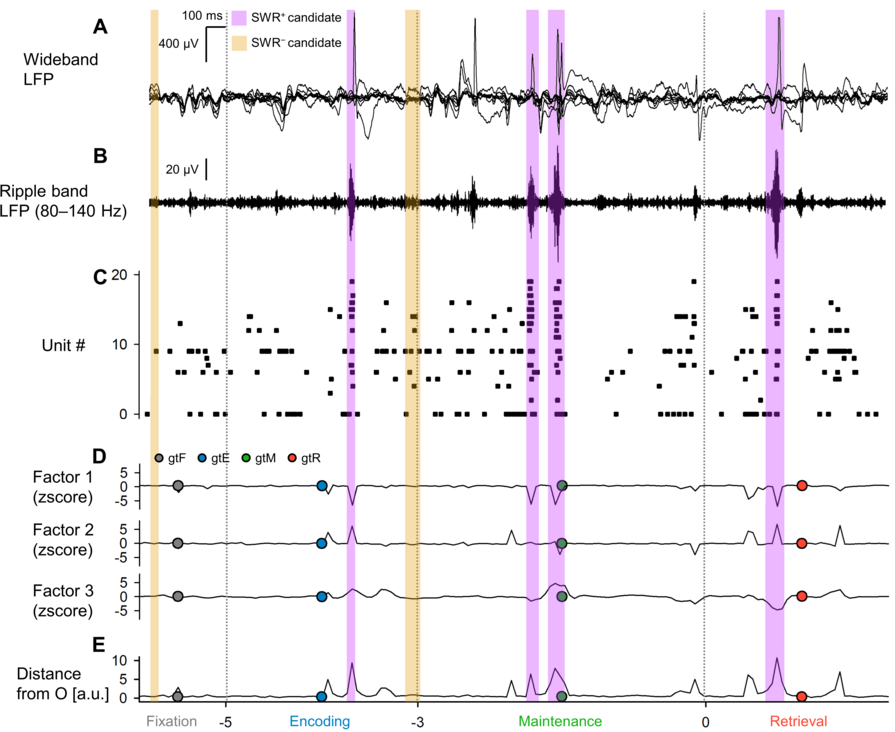
\includegraphics[width=1\textwidth]{./src/figures/.png/Figure_ID_01.png}
        	\caption{\DIFdelbeginFL \textbf{\DIFdelFL{Local Field Potentials (LFP), Multiunit Activity, and Neural Trajectories in the Hippocampus During a Modified Sternberg Task
}}
%DIFAUXCMD
\DIFdelendFL \DIFaddbeginFL \textbf{\DIFaddFL{Local Field Potential (LFP), Multiunit Activity, and Neural Trajectory of the Hippocampus during a Modified Sternberg Task}} \DIFaddFL{\mbox{%DIFAUXCMD
\cite{li_functional_2023, borders_hippocampal_2022, dimakopoulos_information_2022}}\hspace{0pt}%DIFAUXCMD
}}
\DIFaddendFL \smallskip
\\
\textbf{\textit{A.}} \DIFdelbeginFL \DIFdelFL{These traces show representative wideband LFP intracranial EEG (iEEG) signals recorded from the left hippocampal head. The subject performed a modified Sternberg working memory task, which includes fixation (}\DIFdelendFL \DIFaddbeginFL \DIFaddFL{This segment presents representative wideband LFP traces from iEEG signals, observed in the left hippocampal head throughout the completion of a modified Sternberg working memory task. The task involves fixation (}\DIFaddendFL 1 \DIFdelbeginFL \DIFdelFL{s, }\DIFdelendFL \DIFaddbeginFL \DIFaddFL{s, }\DIFaddendFL \textit{gray}\DIFdelbeginFL \DIFdelFL{), encoding (}\DIFdelendFL \DIFaddbeginFL \DIFaddFL{), encoding (}\DIFaddendFL 2 \DIFdelbeginFL \DIFdelFL{s, }\DIFdelendFL \DIFaddbeginFL \DIFaddFL{s, }\DIFaddendFL \textit{blue}\DIFdelbeginFL \DIFdelFL{), maintenance (}\DIFdelendFL \DIFaddbeginFL \DIFaddFL{), maintenance (}\DIFaddendFL 3 \DIFdelbeginFL \DIFdelFL{s, }\DIFdelendFL \DIFaddbeginFL \DIFaddFL{s, }\DIFaddendFL \textit{green}\DIFdelbeginFL \DIFdelFL{), and retrieval (}\DIFdelendFL \DIFaddbeginFL \DIFaddFL{), and retrieval (}\DIFaddendFL 2 \DIFdelbeginFL \DIFdelFL{s, }\DIFdelendFL \DIFaddbeginFL \DIFaddFL{s, }\DIFaddendFL \textit{red}\DIFdelbeginFL \DIFdelFL{). }\DIFdelendFL \DIFaddbeginFL \DIFaddFL{) \mbox{%DIFAUXCMD
\cite{li_functional_2023, borders_hippocampal_2022, dimakopoulos_information_2022}}\hspace{0pt}%DIFAUXCMD
. }\DIFaddendFL \textbf{\textit{B.}} \DIFdelbeginFL \DIFdelFL{We then present the corresponding ripple band LFP traces. }\DIFdelendFL \DIFaddbeginFL \DIFaddFL{The corresponding ripple band LFP traces are depicted here \mbox{%DIFAUXCMD
\cite{schomburg_spiking_2012, behrens_induction_2005, norimoto_hippocampal_2018}}\hspace{0pt}%DIFAUXCMD
. }\DIFaddendFL \textbf{\textit{C.}} \DIFdelbeginFL \DIFdelFL{The raster plot depicts multiunit spikes taken from the LFP traces, sorted using a spike algorithm \mbox{%DIFAUXCMD
\cite{niediek_reliable_2016}}\hspace{0pt}%DIFAUXCMD
. }\DIFdelendFL \DIFaddbeginFL \DIFaddFL{The raster plot of multiunit spikes, derived from the LFP traces utilizing a spike sorting algorithm, is illustrated here \mbox{%DIFAUXCMD
\cite{niediek_reliable_2016}}\hspace{0pt}%DIFAUXCMD
. }\DIFaddendFL \textbf{\textit{D.}} \DIFdelbeginFL \DIFdelFL{Subsequently, we illustrate the neural trajectories, which are calculated by GPFA on spike counts per unit with }\DIFdelendFL \DIFaddbeginFL \DIFaddFL{This part represents the neural trajectory, established by the GPFA, computed from the spike counts per unit within }\DIFaddendFL 50-ms \DIFdelbeginFL \DIFdelFL{bins. Each phase's geometric median is marked by the dot circles. }\DIFdelendFL \DIFaddbeginFL \DIFaddFL{bins \mbox{%DIFAUXCMD
\cite{yu_gaussian-process_2009}}\hspace{0pt}%DIFAUXCMD
. The dotted circles represent the geometric median coordinates for each phase. }\DIFaddendFL \textbf{\textit{E.}} \DIFdelbeginFL \DIFdelFL{The trajectory's distance from the origin }\DIFdelendFL \DIFaddbeginFL \DIFaddFL{The distance from the trajectory to the point }\DIFaddendFL $O$ \DIFdelbeginFL \DIFdelFL{is portrayed, with }\DIFdelendFL \DIFaddbeginFL \DIFaddFL{is demonstrated here. It is notable that the }\DIFaddendFL \textit{purple} and \textit{yellow} \DIFdelbeginFL \DIFdelFL{rectangles indicating the timings for SWR}\DIFdelendFL \DIFaddbeginFL \DIFaddFL{rectangles denote the timings for SWR}\DIFaddendFL $^+$ \DIFdelbeginFL \DIFdelFL{candidates and SWR}\DIFdelendFL \DIFaddbeginFL \DIFaddFL{candidates and SWR}\DIFaddendFL $^-$ \DIFdelbeginFL \DIFdelFL{candidates (considered as controls for SWR}\DIFdelendFL \DIFaddbeginFL \DIFaddFL{candidates, respectively, functioning as controls for SWR}\DIFaddendFL $^+$ \DIFdelbeginFL \DIFdelFL{), respectively.
}%DIFDELCMD < \MBLOCKRIGHTBRACE
%DIFDELCMD < %%%
\DIFdelendFL \DIFaddbeginFL \DIFaddFL{\mbox{%DIFAUXCMD
\cite{van_vugt_hippocampal_2010, scoville_loss_1957, kay_hippocampal_2016, nader_memory_2003, wilson_reactivation_1994, nadasdy_replay_1999, lee_memory_2002}}\hspace{0pt}%DIFAUXCMD
.
}}
\DIFaddendFL % width=1\textwidth
        	\label{fig:01}
        \end{figure*}
        \clearpage
        \begin{figure*}[ht]
            \pdfbookmark[2]{ID 02}{figure_id_02}
        	\centering
            \DIFdelbeginFL %DIFDELCMD < \includegraphics[width=0.5\textwidth]{./src/figures/.png/Figure_ID_02.png}
%DIFDELCMD <         	%%%
\DIFdelendFL \DIFaddbeginFL \includegraphics[width=]{./src/figures/.png/Figure_ID_02.png}
        	\DIFaddendFL \caption{\DIFdelbeginFL \textbf{\DIFdelFL{State-Dependent Trajectories of Hippocampal Neurons
}}
%DIFAUXCMD
\DIFdelendFL \DIFaddbeginFL \textbf{
\DIFaddFL{State-dependent Hippocampal Neural Trajectory
}}
\DIFaddendFL \smallskip
\\
\textbf{\textit{A.}} \DIFdelbeginFL \DIFdelFL{Neural trajectories }\DIFdelendFL \DIFaddbeginFL \DIFaddFL{This figure presents the neural trajectory }\DIFaddendFL within the \DIFdelbeginFL \DIFdelFL{initial three-dimensional factors }\DIFdelendFL \DIFaddbeginFL \DIFaddFL{first three dimensions, }\DIFaddendFL derived \DIFdelbeginFL \DIFdelFL{from the }\DIFdelendFL \DIFaddbeginFL \DIFaddFL{using }\DIFaddendFL Gaussian Process Factor Analysis (GPFA)\DIFdelbeginFL \DIFdelFL{are displayed}\DIFdelendFL . \DIFdelbeginFL \DIFdelFL{The }\DIFdelendFL \DIFaddbeginFL \DIFaddFL{Each }\DIFaddendFL smaller \DIFdelbeginFL \DIFdelFL{dots correspond to }\DIFdelendFL \DIFaddbeginFL \DIFaddFL{dot signifies the }\DIFaddendFL coordinates of \DIFaddbeginFL \DIFaddFL{a }\DIFaddendFL 50-ms neural trajectory \DIFdelbeginFL \DIFdelFL{bins}\DIFdelendFL \DIFaddbeginFL \DIFaddFL{bin}\DIFaddendFL , while \DIFdelbeginFL \DIFdelFL{the }\DIFdelendFL larger dots \DIFdelbeginFL \DIFdelFL{with }\DIFdelendFL \DIFaddbeginFL \DIFaddFL{indicated in }\DIFaddendFL \textit{black} \DIFdelbeginFL \DIFdelFL{edges signify }\DIFdelendFL \DIFaddbeginFL \DIFaddFL{represent }\DIFaddendFL the geometric medians \DIFdelbeginFL \DIFdelFL{for respective stages }\DIFdelendFL \DIFaddbeginFL \DIFaddFL{of successive phases }\DIFaddendFL in the Sternberg working memory task\DIFdelbeginFL \DIFdelFL{: }\DIFdelendFL \DIFaddbeginFL \DIFaddFL{. The phases include }\DIFaddendFL fixation (\textit{gray}), encoding (\textit{blue}), maintenance (\textit{green}), and retrieval (\textit{red})\DIFaddbeginFL \DIFaddFL{\mbox{%DIFAUXCMD
\cite{yu_gaussian-process_2009}}\hspace{0pt}%DIFAUXCMD
}\DIFaddendFL . \textbf{\textit{B.}} The \DIFdelbeginFL \DIFdelFL{figure conveys }\DIFdelendFL \DIFaddbeginFL \DIFaddFL{graph shows }\DIFaddendFL the log-likelihood of \DIFdelbeginFL \DIFdelFL{the }\DIFdelendFL GPFA models \DIFdelbeginFL \DIFdelFL{versus }\DIFdelendFL \DIFaddbeginFL \DIFaddFL{compared to }\DIFaddendFL the \DIFdelbeginFL \DIFdelFL{count }\DIFdelendFL \DIFaddbeginFL \DIFaddFL{number }\DIFaddendFL of dimensions \DIFdelbeginFL \DIFdelFL{used to embed multiunit }\DIFdelendFL \DIFaddbeginFL \DIFaddFL{employed for embedding multi-unit }\DIFaddendFL spikes \DIFdelbeginFL \DIFdelFL{found in the }\DIFdelendFL \DIFaddbeginFL \DIFaddFL{within }\DIFaddendFL medial temporal lobe (MTL) \DIFdelbeginFL \DIFdelFL{territories}\DIFdelendFL \DIFaddbeginFL \DIFaddFL{regions}\DIFaddendFL . \DIFdelbeginFL \DIFdelFL{In specific}\DIFdelendFL \DIFaddbeginFL \DIFaddFL{Notably}\DIFaddendFL , the \DIFdelbeginFL \DIFdelFL{elbow method pinpointed the }\DIFdelendFL optimal \DIFdelbeginFL \DIFdelFL{dimension }\DIFdelendFL \DIFaddbeginFL \DIFaddFL{dimensionality was found }\DIFaddendFL to be three\DIFaddbeginFL \DIFaddFL{, based on the elbow method\mbox{%DIFAUXCMD
\cite{virtanen_scipy_2020}}\hspace{0pt}%DIFAUXCMD
}\DIFaddendFL . \textbf{\textit{C.}} This \DIFdelbeginFL \DIFdelFL{panel illustrates }\DIFdelendFL \DIFaddbeginFL \DIFaddFL{section delineates }\DIFaddendFL the distance \DIFdelbeginFL \DIFdelFL{of }\DIFdelendFL \DIFaddbeginFL \DIFaddFL{between }\DIFaddendFL the neural \DIFdelbeginFL \DIFdelFL{trajectories from }\DIFdelendFL \DIFaddbeginFL \DIFaddFL{trajectory and }\DIFaddendFL the origin ($O$) for the hippocampus (Hipp.), entorhinal cortex (EC), and amygdala (Amy.), \DIFdelbeginFL \DIFdelFL{against the }\DIFdelendFL \DIFaddbeginFL \DIFaddFL{and plots it over }\DIFaddendFL time \DIFdelbeginFL \DIFdelFL{elapsed from }\DIFdelendFL \DIFaddbeginFL \DIFaddFL{since }\DIFaddendFL the \DIFdelbeginFL \DIFdelFL{probe }\DIFdelendFL onset \DIFaddbeginFL \DIFaddFL{of the probe \mbox{%DIFAUXCMD
\cite{boran_dataset_2020}}\hspace{0pt}%DIFAUXCMD
}\DIFaddendFL . \textbf{\textit{D.}} The \DIFdelbeginFL \DIFdelFL{distance of }\DIFdelendFL \DIFaddbeginFL \DIFaddFL{subsequent graph underscores }\DIFaddendFL the trajectory\DIFaddbeginFL \DIFaddFL{'s distance }\DIFaddendFL from $O$ \DIFdelbeginFL \DIFdelFL{within }\DIFdelendFL \DIFaddbeginFL \DIFaddFL{across }\DIFaddendFL MTL regions\DIFdelbeginFL \DIFdelFL{is displayed. The }\DIFdelendFL \DIFaddbeginFL \DIFaddFL{, with the }\DIFaddendFL hippocampus \DIFdelbeginFL \DIFdelFL{shows }\DIFdelendFL \DIFaddbeginFL \DIFaddFL{registering }\DIFaddendFL the \DIFdelbeginFL \DIFdelFL{farthest }\DIFdelendFL \DIFaddbeginFL \DIFaddFL{most extensive }\DIFaddendFL distance, followed by the EC and \DIFdelbeginFL \DIFdelFL{the }\DIFdelendFL Amygdala\DIFaddbeginFL \DIFaddFL{\mbox{%DIFAUXCMD
\cite{fernandez-ruiz_long-duration_2019}}\hspace{0pt}%DIFAUXCMD
}\DIFaddendFL . \textbf{\textit{E.}} The \DIFdelbeginFL \DIFdelFL{plot represents }\DIFdelendFL \DIFaddbeginFL \DIFaddFL{final depiction signifies the }\DIFaddendFL inter-phase trajectory distances within the MTL regions\DIFaddbeginFL \DIFaddFL{\mbox{%DIFAUXCMD
\cite{liu_consensus_2022}}\hspace{0pt}%DIFAUXCMD
}\DIFaddendFL .
Abbreviations:
}
        	%DIF <  width=0.5\textwidth
        	\label{fig:02}
        \end{figure*}
        \clearpage
        \begin{figure*}[ht]
            \pdfbookmark[2]{ID 03}{figure_id_03}
        	\centering
            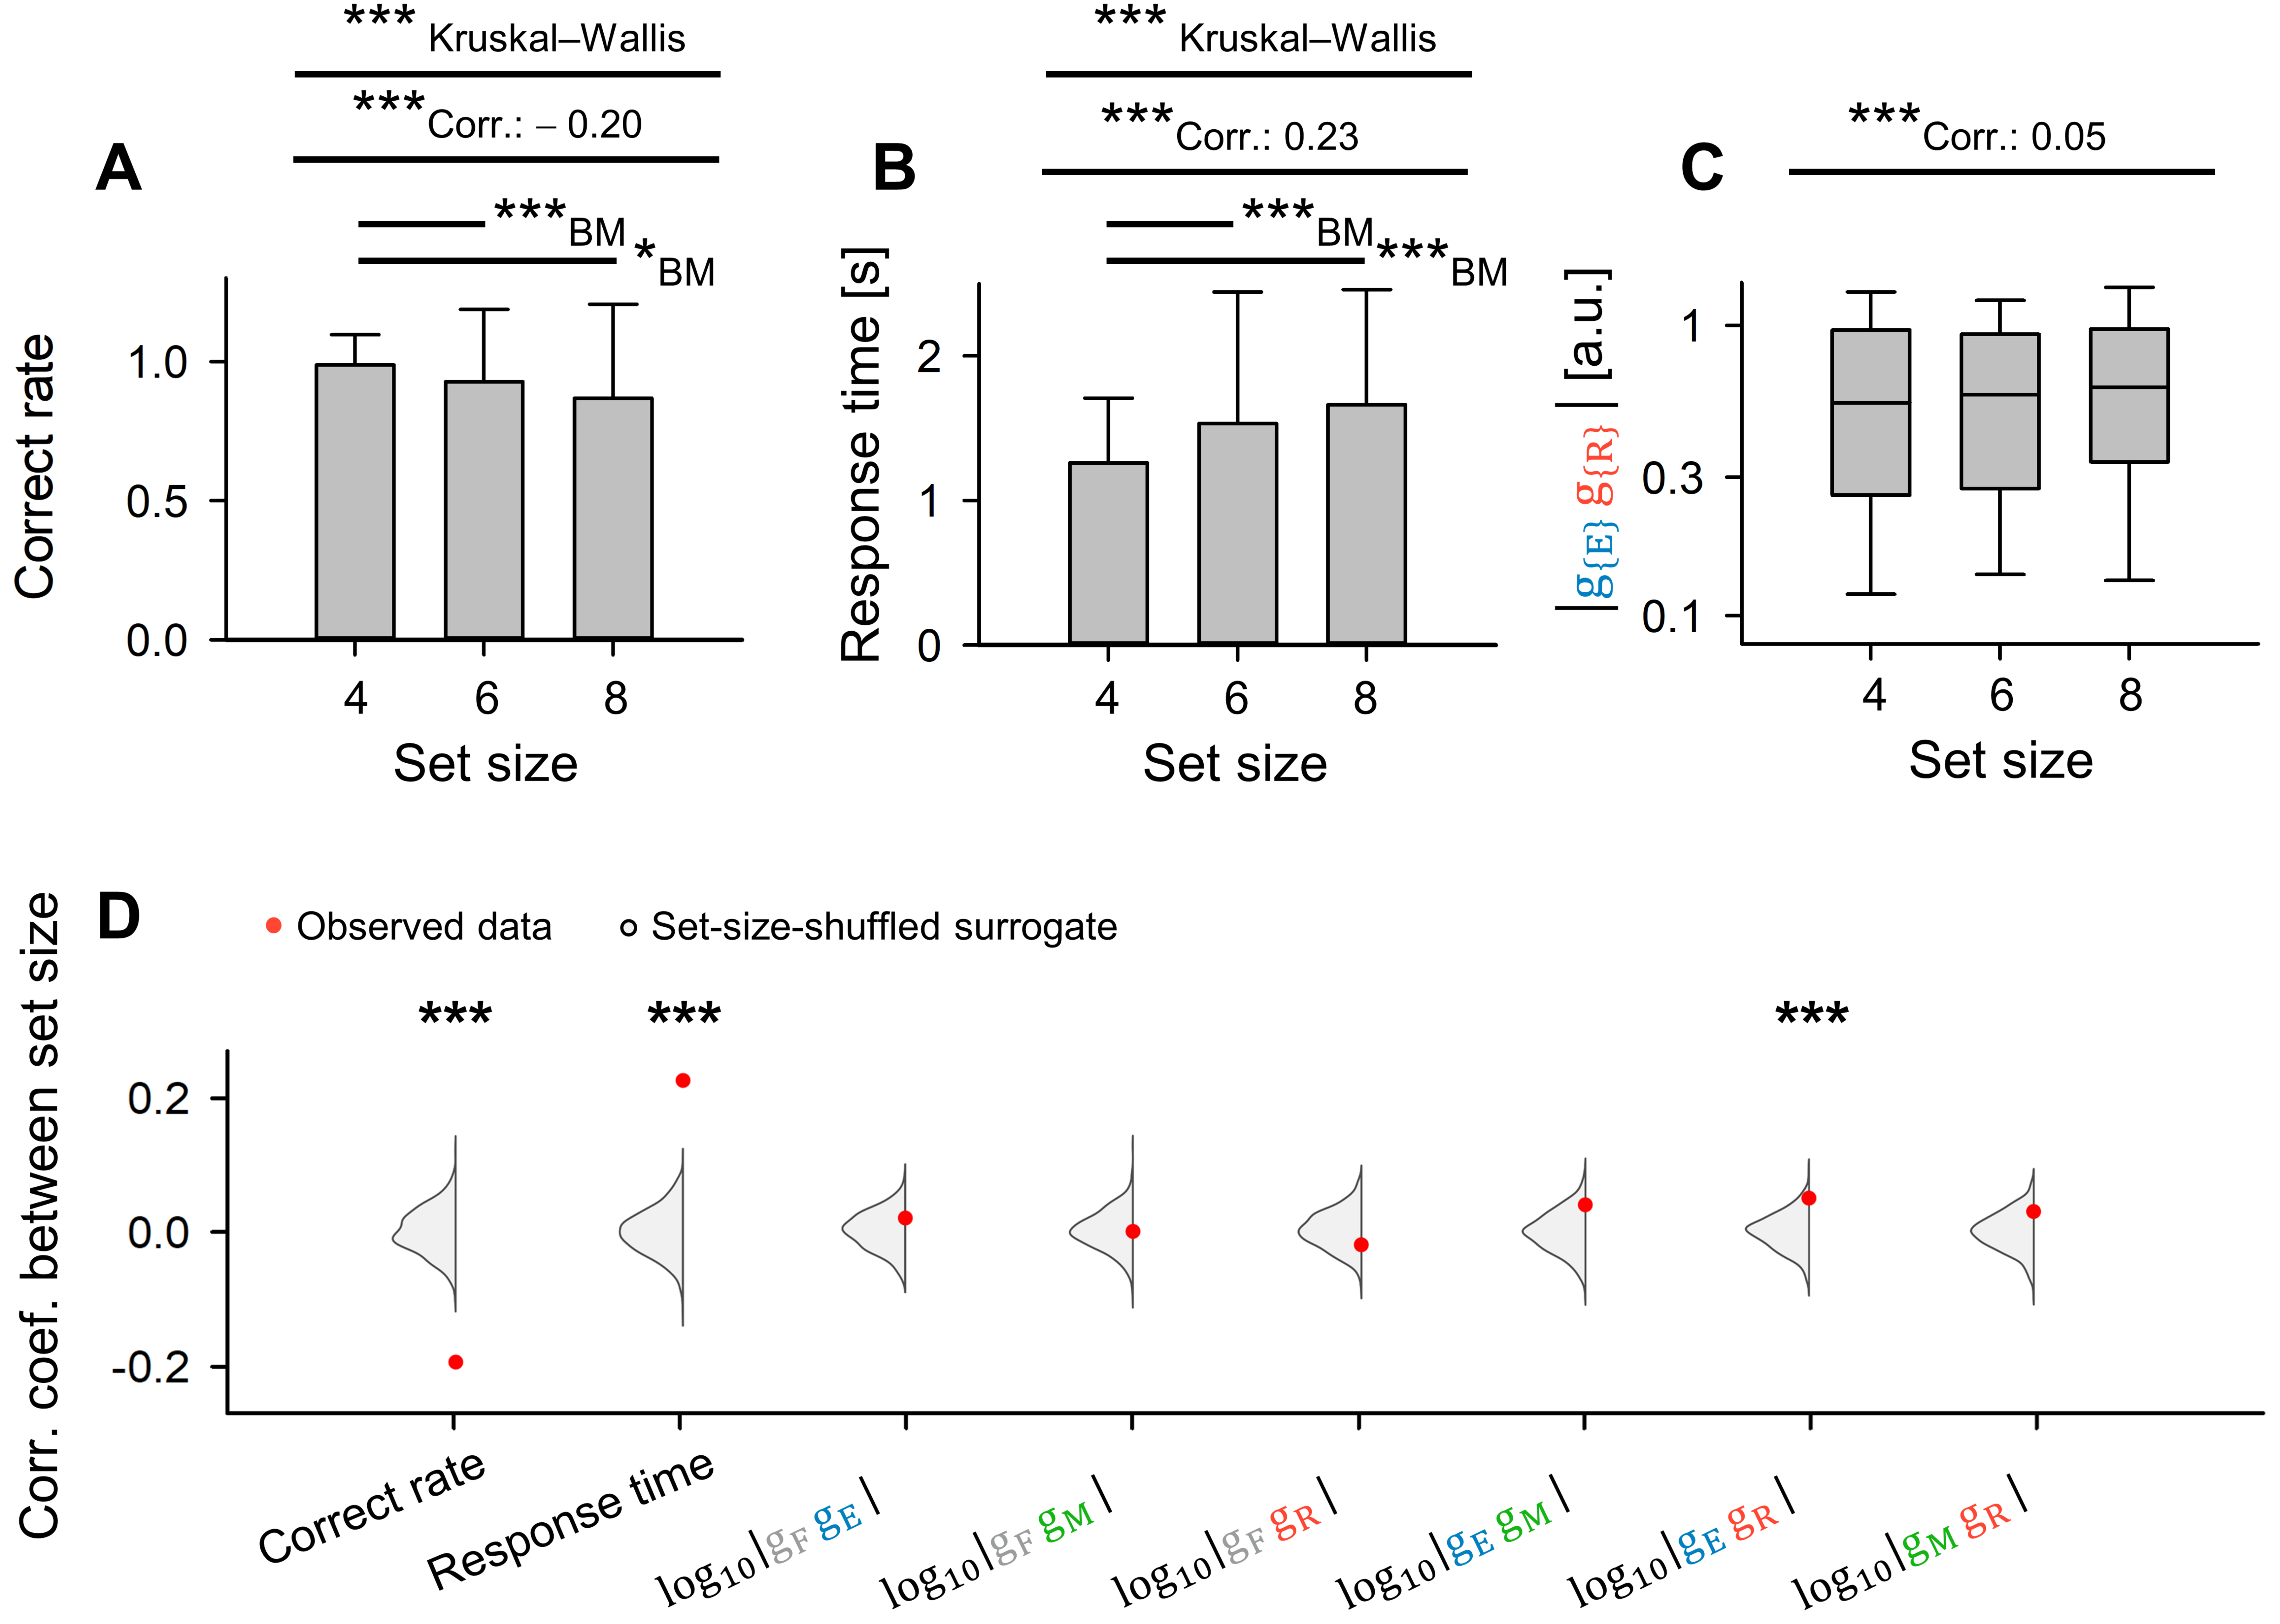
\includegraphics[width=1\textwidth]{./src/figures/.png/Figure_ID_03.png}
        	\caption{\DIFdelbeginFL \textbf{\DIFdelFL{Dependency of Trajectory Distance on Memory Load: Encoding and Retrieval States in Hippocampus
}}
%DIFAUXCMD
\DIFdelendFL \DIFaddbeginFL \textbf{
\DIFaddFL{Dependence of Trajectory Distance on Memory Load Between Encoding and Retrieval States in the Hippocampus
}}
\DIFaddendFL \smallskip
\\
\textbf{\textit{A.}} \DIFdelbeginFL \DIFdelFL{The relationship }\DIFdelendFL \DIFaddbeginFL \DIFaddFL{A significant correlation has been documented }\DIFaddendFL between \DIFaddbeginFL \DIFaddFL{the }\DIFaddendFL set size (\DIFaddbeginFL \DIFaddFL{the }\DIFaddendFL number of letters \DIFdelbeginFL \DIFdelFL{that need }\DIFdelendFL to \DIFdelbeginFL \DIFdelFL{be encoded}\DIFdelendFL \DIFaddbeginFL \DIFaddFL{encode}\DIFaddendFL ) and \DIFdelbeginFL \DIFdelFL{correct }\DIFdelendFL \DIFaddbeginFL \DIFaddFL{the correctness }\DIFaddendFL rate in the \DIFdelbeginFL \DIFdelFL{working memory }\DIFdelendFL \DIFaddbeginFL \DIFaddFL{WM }\DIFaddendFL task (coefficient = $-0.20$, ***\textit{p} $<$ 0.001) \DIFaddbeginFL \DIFaddFL{\mbox{%DIFAUXCMD
\cite{van_vugt_hippocampal_2010, li_functional_2023, borders_hippocampus_2022}}\hspace{0pt}%DIFAUXCMD
}\DIFaddendFL . \textbf{\textit{B.}} \DIFdelbeginFL \DIFdelFL{The }\DIFdelendFL \DIFaddbeginFL \DIFaddFL{A notable }\DIFaddendFL correlation \DIFaddbeginFL \DIFaddFL{exists }\DIFaddendFL between set size and response time (coefficient = \DIFdelbeginFL \DIFdelFL{0.23}\DIFdelendFL \DIFaddbeginFL \DIFaddFL{$0.23$}\DIFaddendFL , ***\textit{p} $<$ 0.001) \DIFaddbeginFL \DIFaddFL{\mbox{%DIFAUXCMD
\cite{dimakopoulos_information_2022}}\hspace{0pt}%DIFAUXCMD
}\DIFaddendFL .  \textbf{\textit{C.}} \DIFdelbeginFL \DIFdelFL{The impact of }\DIFdelendFL \DIFaddbeginFL \DIFaddFL{There is a correlation between }\DIFaddendFL set size \DIFdelbeginFL \DIFdelFL{on }\DIFdelendFL \DIFaddbeginFL \DIFaddFL{and }\DIFaddendFL the \DIFdelbeginFL \DIFdelFL{inter-phase }\DIFdelendFL distances between \DIFdelbeginFL \DIFdelFL{the }\DIFdelendFL encoding and retrieval phases (\DIFdelbeginFL \DIFdelFL{$\lVert \mathrm{g_{E}g_{R}} \rVert$}\DIFdelendFL \DIFaddbeginFL \DIFaddFL{$\Vert \mathrm{g_{E}g_{R}} \Vert$}\DIFaddendFL )\DIFaddbeginFL \DIFaddFL{, but it's less significant }\DIFaddendFL (correlation coefficient = 0.05) \DIFaddbeginFL \DIFaddFL{\mbox{%DIFAUXCMD
\cite{li_functional_2023}}\hspace{0pt}%DIFAUXCMD
}\DIFaddendFL . \textbf{\textit{D.}} \textit{Red} dots \DIFdelbeginFL \DIFdelFL{represent experimental observations of }\DIFdelendFL \DIFaddbeginFL \DIFaddFL{express the observed }\DIFaddendFL correlations between set size and the \DIFdelbeginFL \DIFdelFL{following }\DIFdelendFL \DIFaddbeginFL \DIFaddFL{stated }\DIFaddendFL parameters: correct rate, response time, \DIFdelbeginFL \DIFdelFL{$\log_{10}{\lVert \mathrm{g_{F}g_{E}} \rVert}$}\DIFdelendFL \DIFaddbeginFL \DIFaddFL{$\log_{10}{\Vert \mathrm{g_{F}g_{E}} \Vert}$}\DIFaddendFL , \DIFdelbeginFL \DIFdelFL{$\log_{10}{\lVert \mathrm{g_{F}g_{M}} \rVert}$}\DIFdelendFL \DIFaddbeginFL \DIFaddFL{$\log_{10}{\Vert \mathrm{g_{F}g_{M}} \Vert}$}\DIFaddendFL , \DIFdelbeginFL \DIFdelFL{$\log_{10}{\lVert \mathrm{g_{F}g_{R}} \rVert}$}\DIFdelendFL \DIFaddbeginFL \DIFaddFL{$\log_{10}{\Vert \mathrm{g_{F}g_{R}} \Vert}$}\DIFaddendFL , \DIFdelbeginFL \DIFdelFL{$\log_{10}{\lVert \mathrm{g_{E}g_{M}} \rVert}$}\DIFdelendFL \DIFaddbeginFL \DIFaddFL{$\log_{10}{\Vert \mathrm{g_{E}g_{M}} \Vert}$}\DIFaddendFL , \DIFdelbeginFL \DIFdelFL{$\log_{10}{\lVert \mathrm{g_{E}g_{R}} \rVert}$}\DIFdelendFL \DIFaddbeginFL \DIFaddFL{$\log_{10}{\Vert \mathrm{g_{E}g_{R}} \Vert}$}\DIFaddendFL , and \DIFdelbeginFL \DIFdelFL{$\log_{10}{\lVert \mathrm{g_{M}g_{R}} \rVert}$}\DIFdelendFL \DIFaddbeginFL \DIFaddFL{$\log_{10}{\Vert \mathrm{g_{M}g_{R}} \Vert}$}\DIFaddendFL . The \textit{gray} kernel density plot illustrates the corresponding \DIFdelbeginFL \DIFdelFL{set-size-shuffled surrogate }\DIFdelendFL \DIFaddbeginFL \DIFaddFL{randomized set-size measurements }\DIFaddendFL (\textit{n} = 1,000) (***\textit{p}s $<$ 0.001) \DIFaddbeginFL \DIFaddFL{\mbox{%DIFAUXCMD
\cite{norimoto_hippocampal_2018, hajos_input-output_2013}}\hspace{0pt}%DIFAUXCMD
}\DIFaddendFL .
}
% width=1\textwidth
        	\label{fig:03}
        \end{figure*}
        \clearpage
        \begin{figure*}[ht]
            \pdfbookmark[2]{ID 04}{figure_id_04}
        	\centering
            \includegraphics[width=1\textwidth]{./src/figures/.png/Figure_ID_04.png}
        	\caption{\DIFdelbeginFL \textbf{\DIFdelFL{Detection of SWRs in Presumptive CA1 Regions
}}
%DIFAUXCMD
\DIFdelendFL \DIFaddbeginFL \textbf{\DIFaddFL{Detection of SWRs in Presumed CA1 Regions}}
\DIFaddendFL \smallskip
\\
\textbf{\textit{A.}} \DIFdelbeginFL \DIFdelFL{Two-dimensional UMAP (}\DIFdelendFL \DIFaddbeginFL \DIFaddFL{A two-dimensional }\DIFaddendFL Uniform Manifold Approximation and Projection \DIFaddbeginFL \DIFaddFL{(UMAP}\DIFaddendFL ) \DIFdelbeginFL \DIFdelFL{\mbox{%DIFAUXCMD
\cite{mcinnes_umap_2018} }\hspace{0pt}%DIFAUXCMD
}\DIFdelendFL projection of \DIFdelbeginFL \DIFdelFL{multiunit }\DIFdelendFL \DIFaddbeginFL \DIFaddFL{multi-unit }\DIFaddendFL spikes during \DIFdelbeginFL \DIFdelFL{SWR$^+$ candidates }\DIFdelendFL \DIFaddbeginFL \DIFaddFL{potential SWRs }\DIFaddendFL (\textit{purple}) and \DIFdelbeginFL \DIFdelFL{SWR$^-$ candidates }\DIFdelendFL \DIFaddbeginFL \DIFaddFL{non-SWRs }\DIFaddendFL (\textit{yellow}) \DIFaddbeginFL \DIFaddFL{periods is given\mbox{%DIFAUXCMD
\cite{mcinnes_umap_2018}}\hspace{0pt}%DIFAUXCMD
}\DIFaddendFL . \textbf{\textit{B.}} \DIFdelbeginFL \DIFdelFL{Cumulative }\DIFdelendFL \DIFaddbeginFL \DIFaddFL{The cumulative }\DIFaddendFL density plot \DIFdelbeginFL \DIFdelFL{shows }\DIFdelendFL \DIFaddbeginFL \DIFaddFL{of }\DIFaddendFL silhouette scores, \DIFdelbeginFL \DIFdelFL{indicative }\DIFdelendFL \DIFaddbeginFL \DIFaddFL{measuring the quality }\DIFaddendFL of UMAP clustering \DIFdelbeginFL \DIFdelFL{quality, for }\DIFdelendFL \DIFaddbeginFL \DIFaddFL{across diverse }\DIFaddendFL hippocampal regions\DIFaddbeginFL \DIFaddFL{, is shown }\DIFaddendFL (\DIFdelbeginFL \DIFdelFL{see }\DIFdelendFL \DIFaddbeginFL \DIFaddFL{refer to }\DIFaddendFL Table~\ref{tab:02}\DIFdelbeginFL \DIFdelFL{for reference}\DIFdelendFL ). \DIFdelbeginFL \DIFdelFL{Note }\DIFdelendFL \DIFaddbeginFL \DIFaddFL{Regions }\DIFaddendFL that \DIFdelbeginFL \DIFdelFL{hippocampal regions with }\DIFdelendFL \DIFaddbeginFL \DIFaddFL{attained a }\DIFaddendFL silhouette \DIFdelbeginFL \DIFdelFL{scores greater than }\DIFdelendFL \DIFaddbeginFL \DIFaddFL{score above }\DIFaddendFL 0.60 (\DIFdelbeginFL \DIFdelFL{equivalent }\DIFdelendFL \DIFaddbeginFL \DIFaddFL{corresponding }\DIFaddendFL to the $75^{th}$ percentile)\DIFdelbeginFL \DIFdelFL{were }\DIFdelendFL \DIFaddbeginFL \DIFaddFL{, are }\DIFaddendFL identified as \DIFdelbeginFL \DIFdelFL{possible }\DIFdelendFL \DIFaddbeginFL \DIFaddFL{probable }\DIFaddendFL CA1 \DIFdelbeginFL \DIFdelFL{regions}\DIFdelendFL \DIFaddbeginFL \DIFaddFL{areas}\DIFaddendFL . \DIFdelbeginFL \DIFdelFL{SWR$^+$ and SWR$^-$ candidates recorded from }\DIFdelendFL \DIFaddbeginFL \DIFaddFL{Within }\DIFaddendFL these \DIFdelbeginFL \DIFdelFL{speculative }\DIFdelendFL \DIFaddbeginFL \DIFaddFL{potential }\DIFaddendFL CA1 regions\DIFaddbeginFL \DIFaddFL{, the SWR and non-SWR periods }\DIFaddendFL were respectively \DIFdelbeginFL \DIFdelFL{classified }\DIFdelendFL \DIFaddbeginFL \DIFaddFL{categorized }\DIFaddendFL as \DIFdelbeginFL \DIFdelFL{SWR$^+$ }\DIFdelendFL \DIFaddbeginFL \DIFaddFL{SWRs }\DIFaddendFL and \DIFdelbeginFL \DIFdelFL{SWR$^-$ }\DIFdelendFL \DIFaddbeginFL \DIFaddFL{non-SWRs }\DIFaddendFL (\textit{n} \DIFdelbeginFL \DIFdelFL{s }\DIFdelendFL = 1,170)\DIFaddbeginFL \DIFaddFL{\mbox{%DIFAUXCMD
\cite{rousseeuw_silhouettes_1987}}\hspace{0pt}%DIFAUXCMD
}\DIFaddendFL . \textbf{\textit{C.}} The \DIFdelbeginFL \DIFdelFL{identical }\DIFdelendFL distributions of durations \DIFdelbeginFL \DIFdelFL{are presented }\DIFdelendFL for \DIFdelbeginFL \DIFdelFL{SWR$^+$ }\DIFdelendFL \DIFaddbeginFL \DIFaddFL{both SWRs }\DIFaddendFL (\textit{purple}) and \DIFdelbeginFL \DIFdelFL{SWR$^-$ }\DIFdelendFL \DIFaddbeginFL \DIFaddFL{non-SWRs }\DIFaddendFL (\textit{yellow}) \DIFaddbeginFL \DIFaddFL{are depicted}\DIFaddendFL , \DIFdelbeginFL \DIFdelFL{owing to }\DIFdelendFL \DIFaddbeginFL \DIFaddFL{based on }\DIFaddendFL their \DIFaddbeginFL \DIFaddFL{respective }\DIFaddendFL definitions (93.0 [65.4] ms, median [IQR])\DIFaddbeginFL \DIFaddFL{\mbox{%DIFAUXCMD
\cite{girardeau_selective_2009}}\hspace{0pt}%DIFAUXCMD
\mbox{%DIFAUXCMD
\cite{norman_hippocampal_2021}}\hspace{0pt}%DIFAUXCMD
}\DIFaddendFL . \textbf{\textit{D.}} \DIFdelbeginFL \DIFdelFL{SWR incidence for both SWR$^+$ }\DIFdelendFL \DIFaddbeginFL \DIFaddFL{An illustration of the frequency of SWRs }\DIFaddendFL (\textit{purple}) and \DIFdelbeginFL \DIFdelFL{SWR$^-$ }\DIFdelendFL \DIFaddbeginFL \DIFaddFL{non-SWRs }\DIFaddendFL (\textit{yellow}) \DIFdelbeginFL \DIFdelFL{obtained relative to }\DIFdelendFL \DIFaddbeginFL \DIFaddFL{over time from }\DIFaddendFL the \DIFdelbeginFL \DIFdelFL{probe's timing is illustrated as a }\DIFdelendFL \DIFaddbeginFL \DIFaddFL{start of stimulation, represented by }\DIFaddendFL mean \DIFaddbeginFL \DIFaddFL{value }\DIFaddendFL \textpm 95\% confidence interval \DIFaddbeginFL \DIFaddFL{is given}\DIFaddendFL . \DIFdelbeginFL \DIFdelFL{However, as the intervals may not }\DIFdelendFL \DIFaddbeginFL \DIFaddFL{It should }\DIFaddendFL be \DIFdelbeginFL \DIFdelFL{visible }\DIFdelendFL \DIFaddbeginFL \DIFaddFL{noted that }\DIFaddendFL due to \DIFdelbeginFL \DIFdelFL{their narrow range}\DIFdelendFL \DIFaddbeginFL \DIFaddFL{close intervals}\DIFaddendFL , \DIFdelbeginFL \DIFdelFL{note that }\DIFdelendFL \DIFaddbeginFL \DIFaddFL{visual differentiation can be difficult. Additionally, there was }\DIFaddendFL a \DIFdelbeginFL \DIFdelFL{significant }\DIFdelendFL \DIFaddbeginFL \DIFaddFL{discernible }\DIFaddendFL increase in SWR \DIFdelbeginFL \DIFdelFL{incidence was detected }\DIFdelendFL \DIFaddbeginFL \DIFaddFL{frequency }\DIFaddendFL during the initial 400 ms of the retrieval phase (0.421 [Hz], *\textit{p} \DIFdelbeginFL \DIFdelFL{$<$ }\DIFdelendFL \DIFaddbeginFL \DIFaddFL{< }\DIFaddendFL 0.05, bootstrap test)\DIFaddbeginFL \DIFaddFL{\mbox{%DIFAUXCMD
\cite{buzsaki_hippocampal_2015}}\hspace{0pt}%DIFAUXCMD
\mbox{%DIFAUXCMD
\cite{ego-stengel_disruption_2010}}\hspace{0pt}%DIFAUXCMD
\mbox{%DIFAUXCMD
\cite{fernandez-ruiz_long-duration_2019}}\hspace{0pt}%DIFAUXCMD
}\DIFaddendFL . \textbf{\textit{E.}} \DIFdelbeginFL \DIFdelFL{The distributions }\DIFdelendFL \DIFaddbeginFL \DIFaddFL{Distributions }\DIFaddendFL of ripple band peak amplitudes for \DIFdelbeginFL \DIFdelFL{SWR$^-$ }\DIFdelendFL \DIFaddbeginFL \DIFaddFL{non-SWRs }\DIFaddendFL (\textit{yellow}; 2.37 [0.33] \DIFaddbeginFL \DIFaddFL{times the standard deviation (}\DIFaddendFL SD\DIFaddbeginFL \DIFaddFL{) }\DIFaddendFL of \DIFaddbeginFL \DIFaddFL{the }\DIFaddendFL baseline, median [IQR]) and \DIFdelbeginFL \DIFdelFL{SWR$^+$ }\DIFdelendFL \DIFaddbeginFL \DIFaddFL{SWRs }\DIFaddendFL (\textit{purple}; 3.05 [0.85] \DIFaddbeginFL \DIFaddFL{times the }\DIFaddendFL SD of \DIFaddbeginFL \DIFaddFL{the }\DIFaddendFL baseline, median [IQR]) are \DIFdelbeginFL \DIFdelFL{delineated }\DIFdelendFL \DIFaddbeginFL \DIFaddFL{exhibited. Considerable differences were observed }\DIFaddendFL (***\textit{p} \DIFdelbeginFL \DIFdelFL{$<$ }\DIFdelendFL \DIFaddbeginFL \DIFaddFL{< }\DIFaddendFL 0.001, \DIFaddbeginFL \DIFaddFL{by }\DIFaddendFL the Brunner--Munzel test)\DIFaddbeginFL \DIFaddFL{\mbox{%DIFAUXCMD
\cite{norman_hippocampal_2019}}\hspace{0pt}%DIFAUXCMD
\mbox{%DIFAUXCMD
\cite{diba_forward_2007}}\hspace{0pt}%DIFAUXCMD
\mbox{%DIFAUXCMD
\cite{liu_consensus_2022}}\hspace{0pt}%DIFAUXCMD
}\DIFaddendFL .
}
% width=1\textwidth
        	\label{fig:04}
        \end{figure*}
        \clearpage
        \begin{figure*}[ht]
            \pdfbookmark[2]{ID 05}{figure_id_05}
        	\centering
            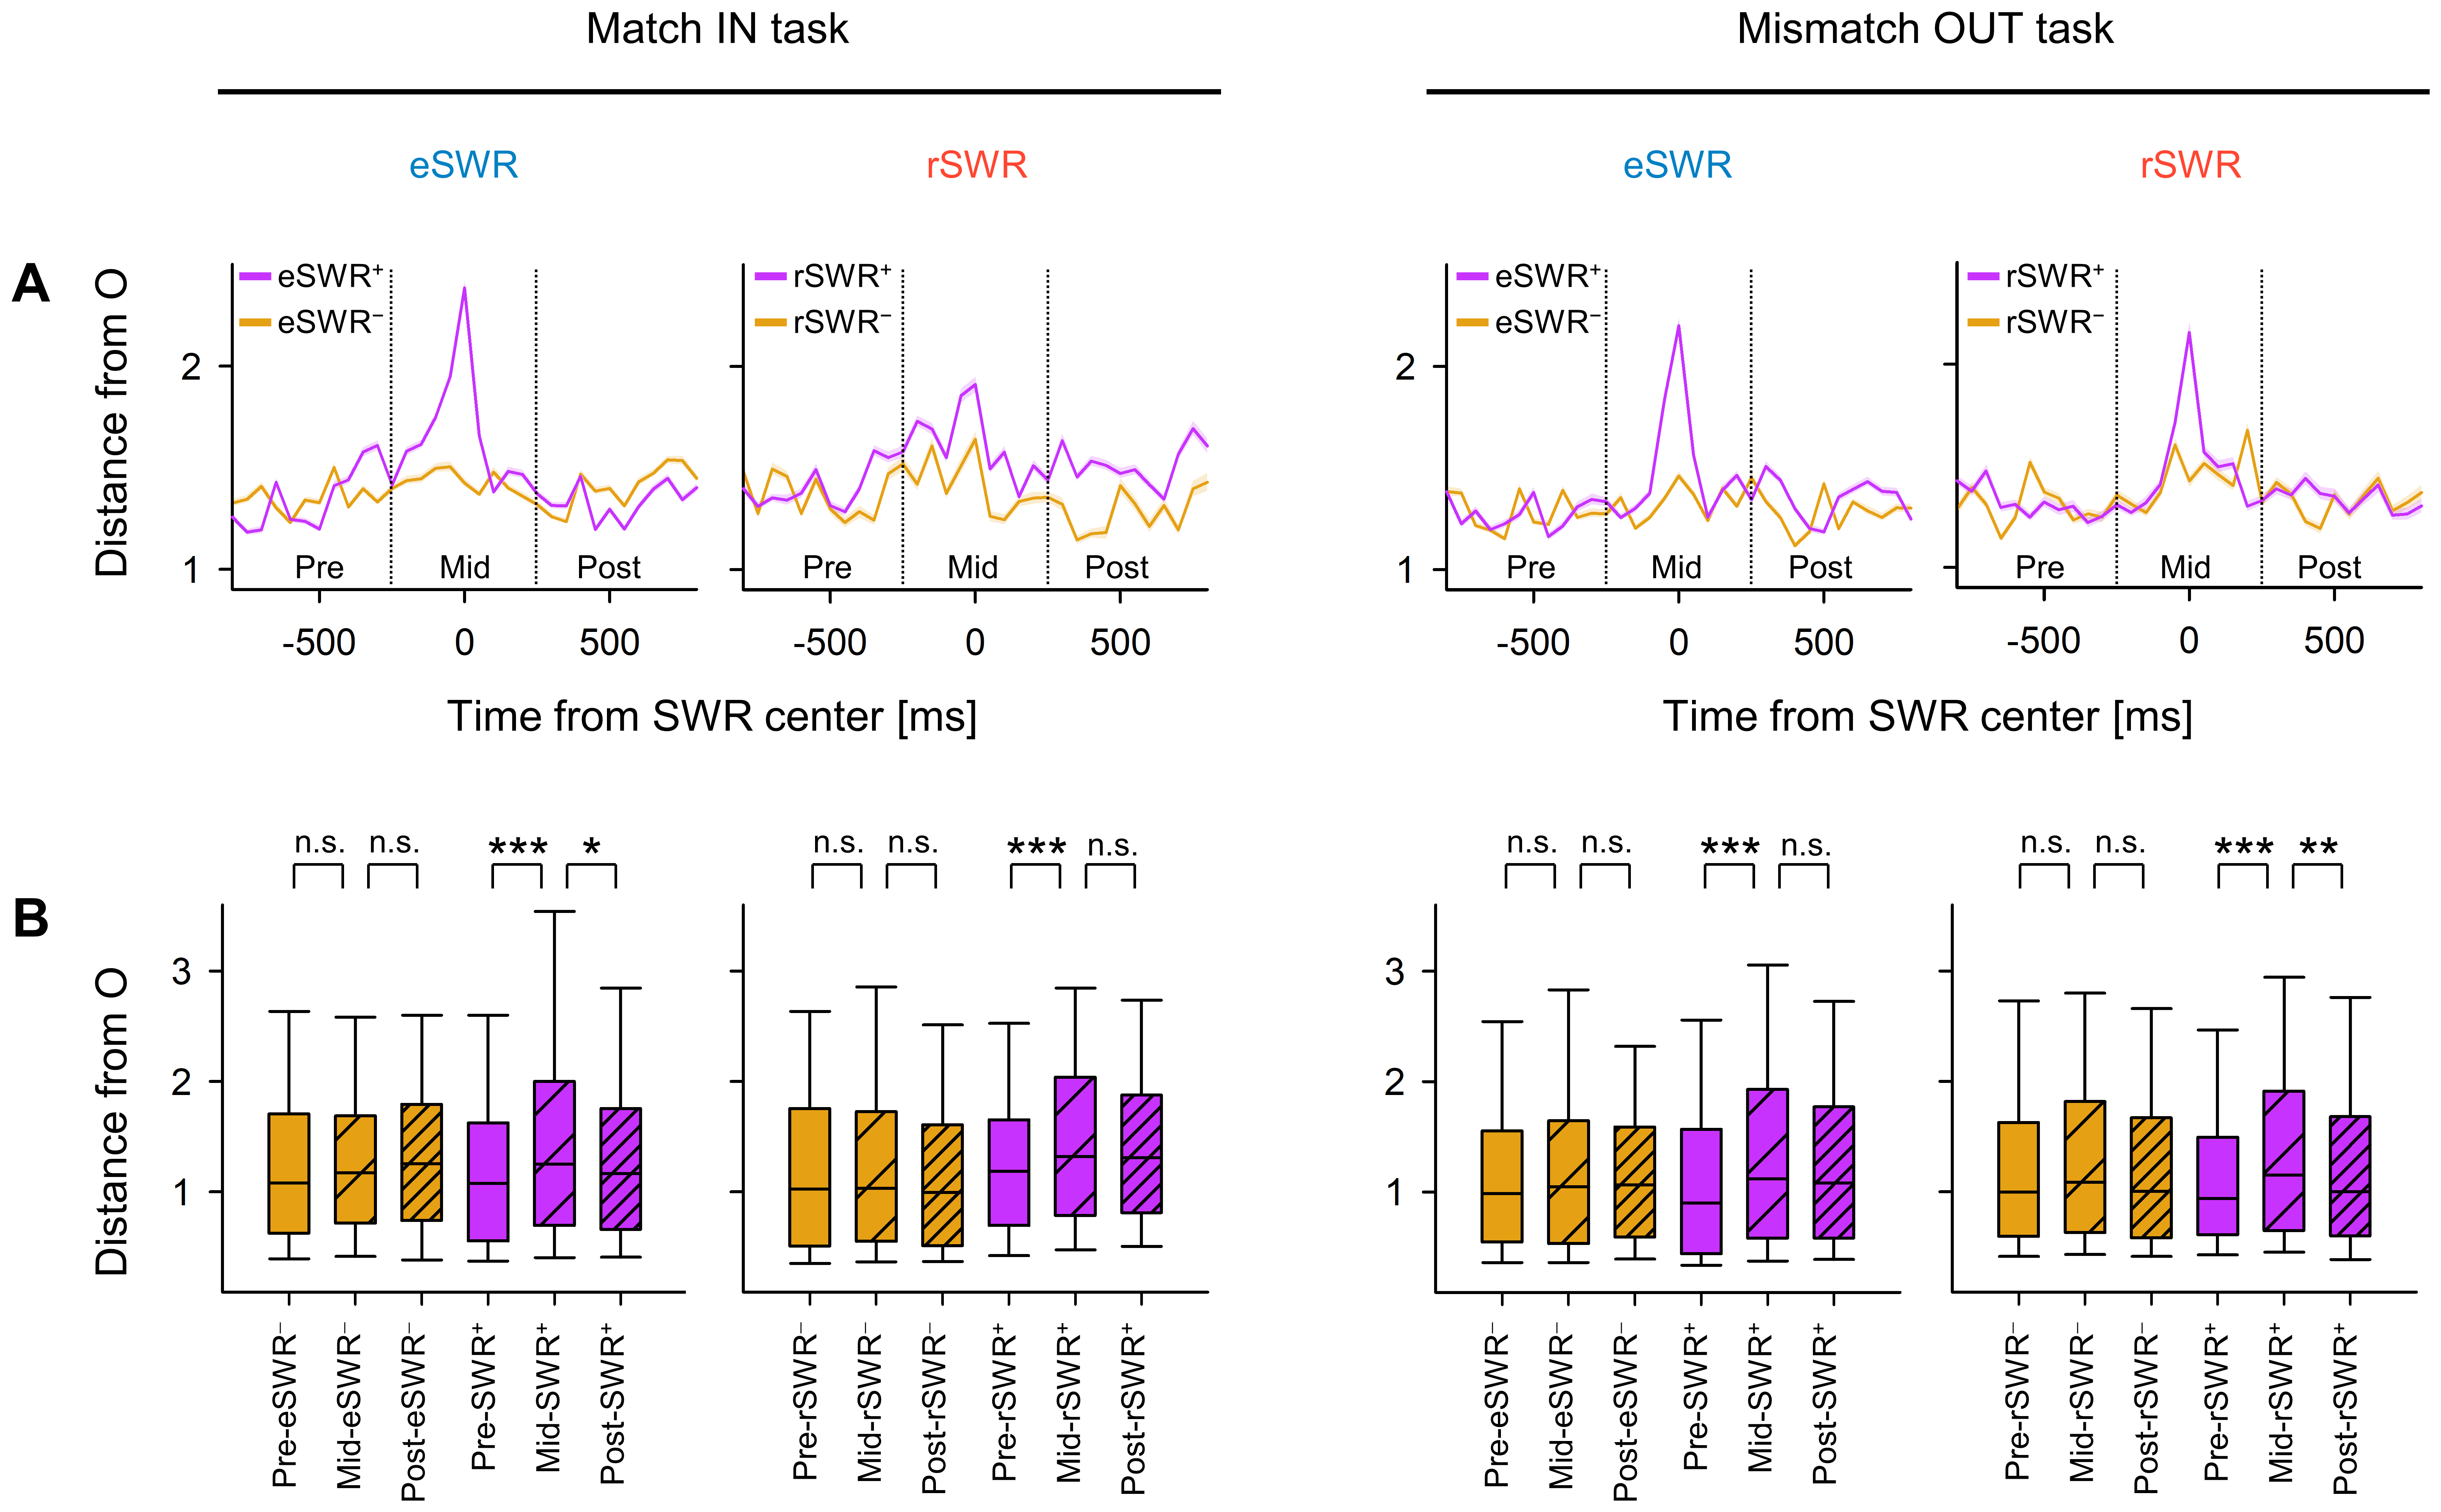
\includegraphics[width=1\textwidth]{./src/figures/.png/Figure_ID_05.png}
        	\caption{\DIFdelbeginFL \textbf{\DIFdelFL{Transient Alterations in Neural Trajectory During SWR Events
}}
%DIFAUXCMD
\DIFdelendFL \DIFaddbeginFL \textbf{\DIFaddFL{Transient Changes in Neural Trajectory During SWR}}}
\DIFaddendFL \smallskip
\\
\textbf{\textit{A.}} \DIFdelbeginFL \DIFdelFL{Displayed is the distance from origin (}\DIFdelendFL \DIFaddbeginFL \DIFaddFL{Depicts the average distance from the origin (}\DIFaddendFL $O$\DIFdelbeginFL \DIFdelFL{) of the }\DIFdelendFL \DIFaddbeginFL \DIFaddFL{) of the }\DIFaddendFL peri-sharp-wave-ripple \DIFdelbeginFL \DIFdelFL{trajectory (mean }%DIFDELCMD < \textpm %%%
\DIFdelendFL \DIFaddbeginFL \DIFaddFL{(SWR) trajectory, alongside a }\DIFaddendFL 95\DIFdelbeginFL \DIFdelFL{\% confidence interval). The intervals may not be apparent due to their slender ranges. }\DIFdelendFL \DIFaddbeginFL \DIFaddFL{\% confidence interval, which may not be evident due to its limited range \mbox{%DIFAUXCMD
\cite{girardeau_selective_2009,norman_hippocampal_2019,buzsaki_hippocampal_2015}}\hspace{0pt}%DIFAUXCMD
. }\DIFaddendFL \textbf{\textit{B.}} \DIFdelbeginFL \DIFdelFL{Shown is the distance from the origin (}\DIFdelendFL \DIFaddbeginFL \DIFaddFL{Demonstrates the distance from the origin (}\DIFaddendFL $O$\DIFdelbeginFL \DIFdelFL{) during }\DIFdelendFL \DIFaddbeginFL \DIFaddFL{) throughout }\DIFaddendFL pre-, mid-\DIFdelbeginFL \DIFdelFL{, and }\DIFdelendFL \DIFaddbeginFL \DIFaddFL{, and }\DIFaddendFL post-SWR \DIFdelbeginFL \DIFdelFL{periods (}\DIFdelendFL \DIFaddbeginFL \DIFaddFL{intervals (}\DIFaddendFL *\textit{p} $<$ 0.05, **\textit{p} $<$ 0.01, ***\textit{p} $<$ 0.001\DIFdelbeginFL \DIFdelFL{; assessed using the }\DIFdelendFL \DIFaddbeginFL \DIFaddFL{; according to the }\DIFaddendFL Brunner--Munzel \DIFdelbeginFL \DIFdelFL{test). Abbreviations: SWR, }\DIFdelendFL \DIFaddbeginFL \DIFaddFL{test \mbox{%DIFAUXCMD
\cite{boran_persistent_2019}}\hspace{0pt}%DIFAUXCMD
). The defined terms are: SWR, }\DIFaddendFL sharp-wave \DIFdelbeginFL \DIFdelFL{ripple events; eSWR, SWR during the encoding phase; rSWR, SWR while in the retrieval phase; SWR}\DIFdelendFL \DIFaddbeginFL \DIFaddFL{ripple events; eSWR, SWR occurring during the encoding phase; rSWR, SWR taking place during the retrieval phase; SWR}\DIFaddendFL $^+$\DIFdelbeginFL \DIFdelFL{, positive SWR event; SWR}\DIFdelendFL \DIFaddbeginFL \DIFaddFL{, an SWR event; SWR}\DIFaddendFL $^-$\DIFdelbeginFL \DIFdelFL{, control events for SWR}\DIFdelendFL \DIFaddbeginFL \DIFaddFL{, the control events aligned with SWR}\DIFaddendFL $^+$; pre-, mid-\DIFdelbeginFL \DIFdelFL{, or }\DIFdelendFL \DIFaddbeginFL \DIFaddFL{, or }\DIFaddendFL post-SWR\DIFdelbeginFL \DIFdelFL{denote the time intervals from }\DIFdelendFL \DIFaddbeginFL \DIFaddFL{, the time segments from }\DIFaddendFL $-800$ to $-250$ \DIFdelbeginFL \DIFdelFL{ms, from }\DIFdelendFL \DIFaddbeginFL \DIFaddFL{ms, from }\DIFaddendFL $-250$ to $+250$ \DIFdelbeginFL \DIFdelFL{ms, or from }\DIFdelendFL \DIFaddbeginFL \DIFaddFL{ms, and from }\DIFaddendFL $+250$ to $+800$ \DIFdelbeginFL \DIFdelFL{ms, all relative to the center of the SWR.
}%DIFDELCMD < \MBLOCKRIGHTBRACE
%DIFDELCMD < %%%
\DIFdelendFL \DIFaddbeginFL \DIFaddFL{ms, respectively, each relative to the SWR center.
}}
\DIFaddendFL % width=1\textwidth
        	\label{fig:05}
        \end{figure*}
        \clearpage
        \begin{figure*}[ht]
            \pdfbookmark[2]{ID 06}{figure_id_06}
        	\centering
            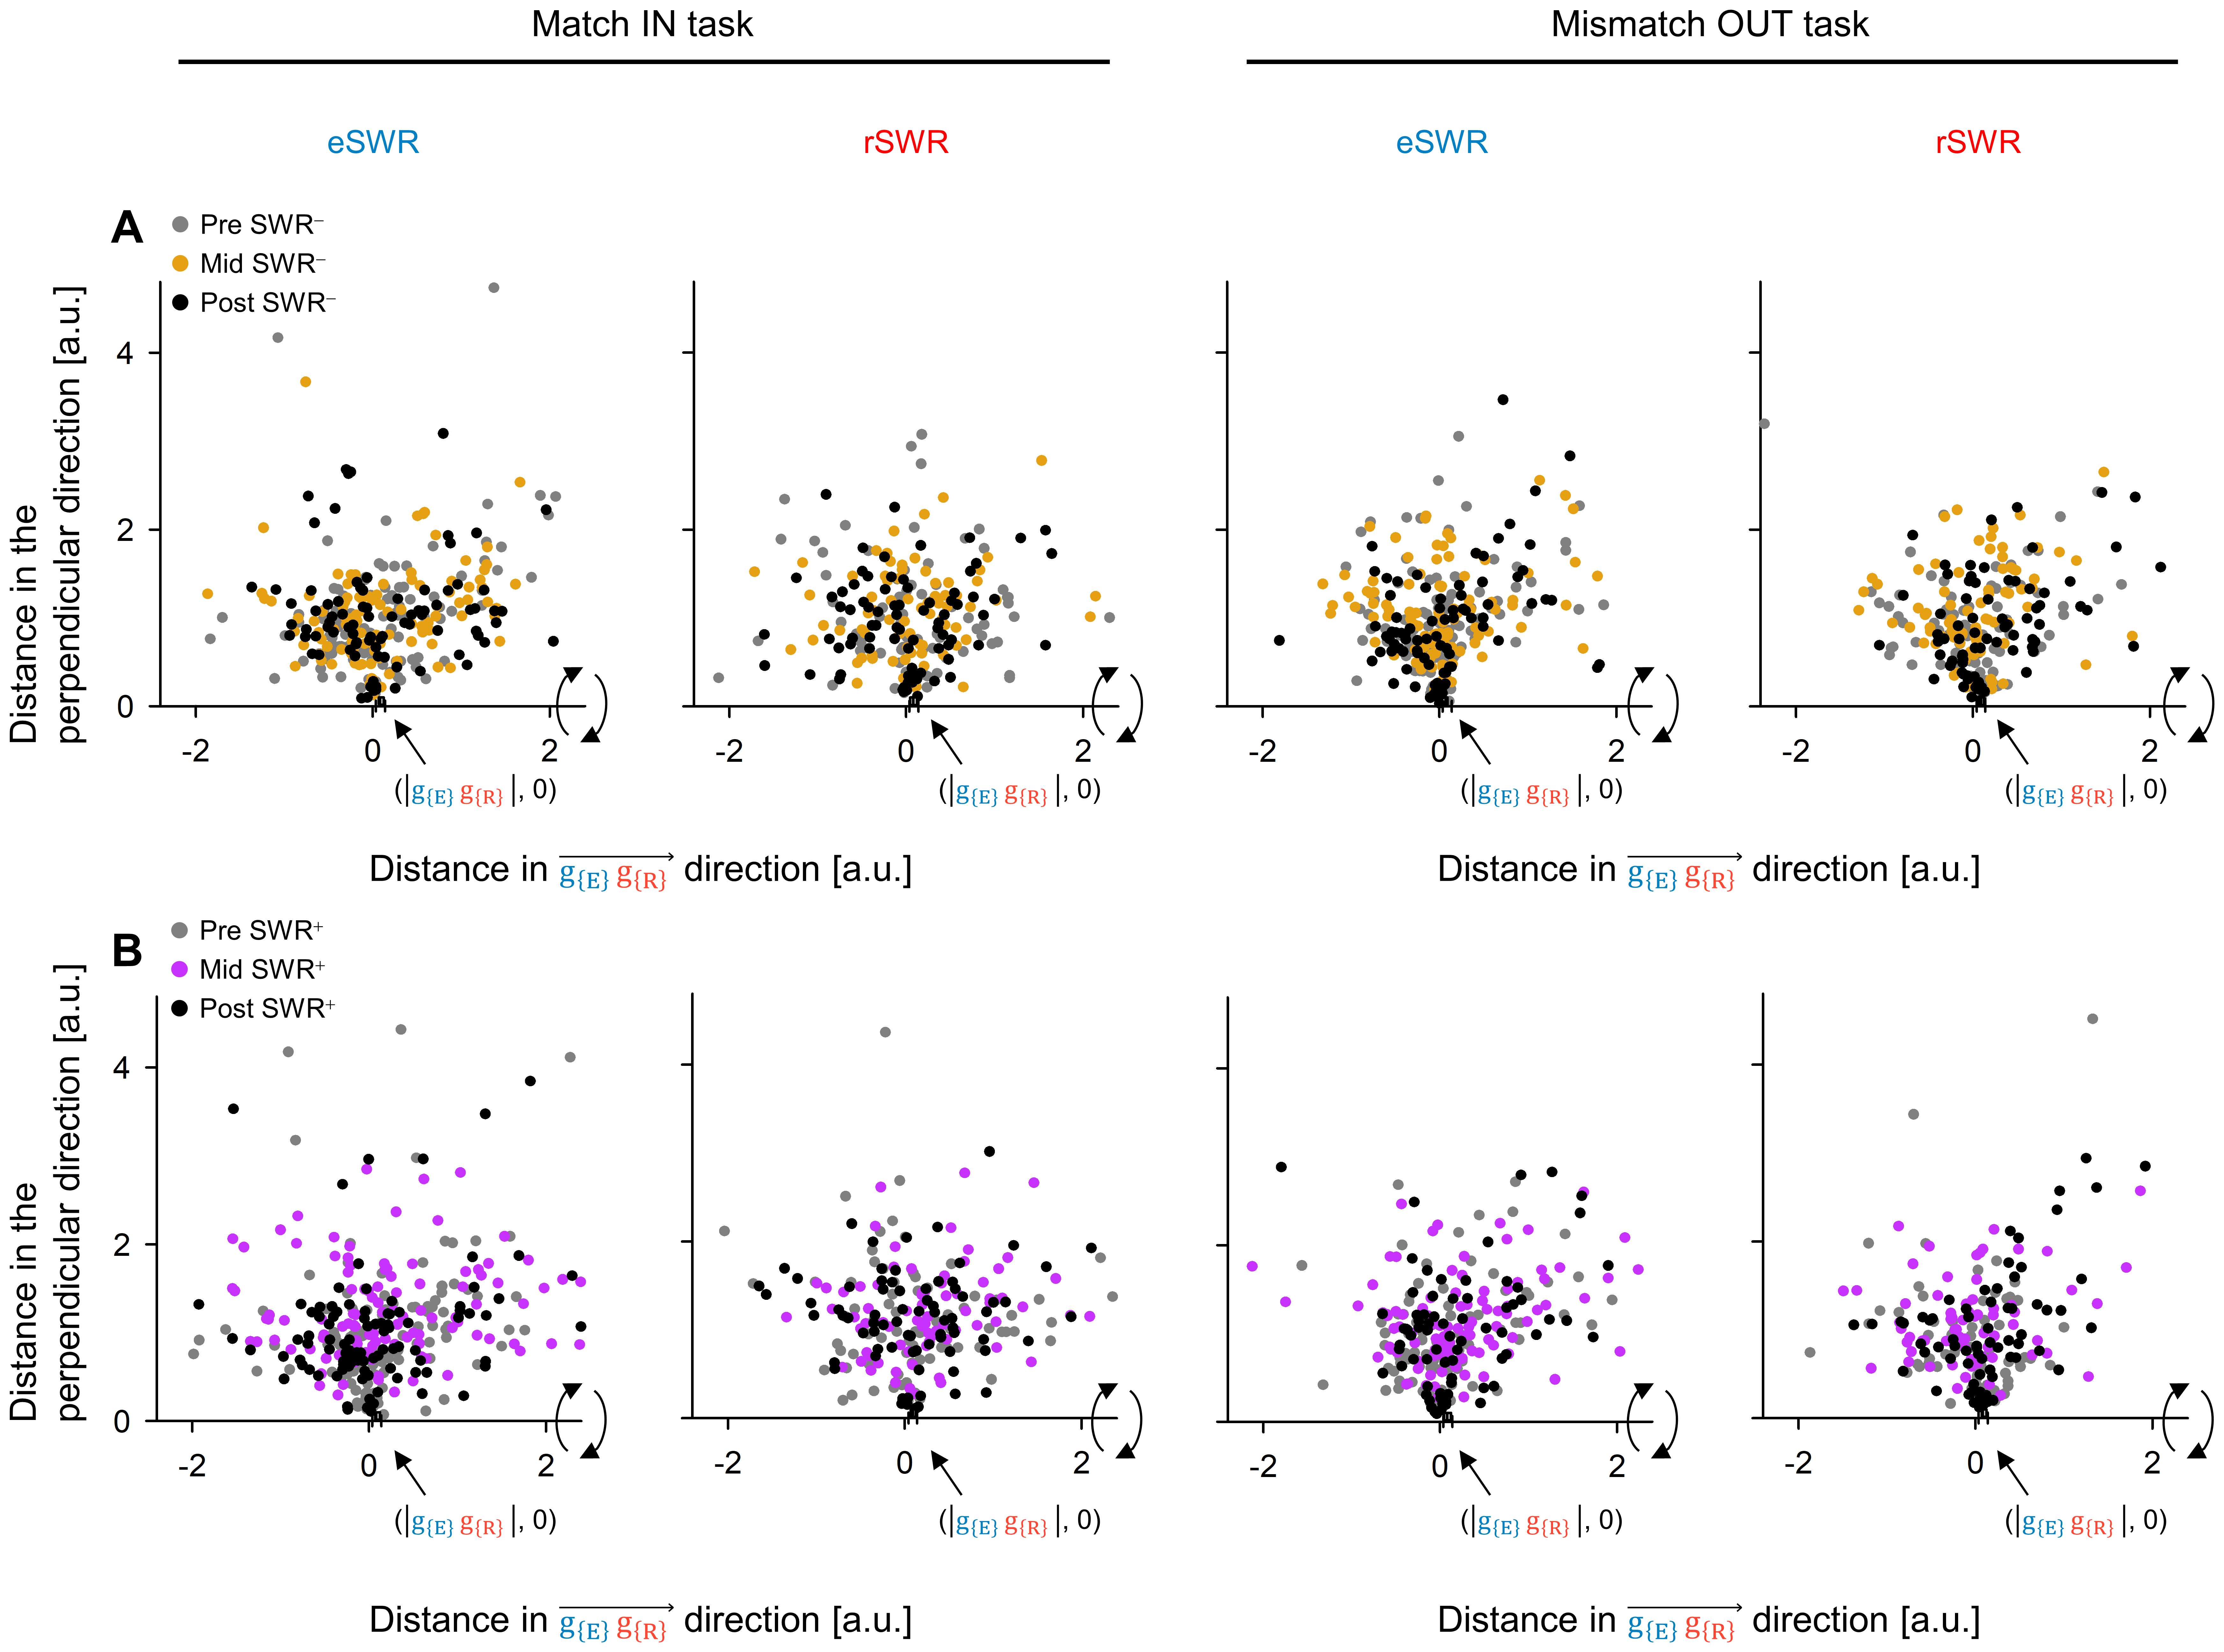
\includegraphics[width=1\textwidth]{./src/figures/.png/Figure_ID_06.png}
        	\caption{\DIFdelbeginFL \textbf{\DIFdelFL{Visualization of Neural Trajectories during SWR in Two-Dimensional Spaces}}
%DIFAUXCMD
\DIFdelendFL \DIFaddbeginFL \textbf{\DIFaddFL{Visualizing Neural Trajectories During Sharp-Wave Ripple Events in a Two-Dimensional Space}}

\DIFaddendFL \smallskip
\DIFaddbeginFL 

\DIFaddendFL \\
\DIFdelbeginFL \DIFdelFL{The panels display hippocampal }\DIFdelendFL \DIFaddbeginFL \DIFaddFL{This figure demonstrates the association of }\DIFaddendFL neural trajectories \DIFaddbeginFL \DIFaddFL{with hippocampal activity }\DIFaddendFL during \DIFaddbeginFL \DIFaddFL{Sharp-Wave Ripple (}\DIFaddendFL SWR\DIFdelbeginFL \DIFdelFL{as projected onto }\DIFdelendFL \DIFaddbeginFL \DIFaddFL{) events in a }\DIFaddendFL two-dimensional \DIFdelbeginFL \DIFdelFL{spaces}\DIFdelendFL \DIFaddbeginFL \DIFaddFL{context}\DIFaddendFL . \textbf{\textit{A.}} \DIFdelbeginFL \DIFdelFL{Indicates hippocampal neural }\DIFdelendFL \DIFaddbeginFL \DIFaddFL{It depicts example }\DIFaddendFL trajectories \DIFdelbeginFL \DIFdelFL{pre-SWR$^-$ }\DIFdelendFL \DIFaddbeginFL \DIFaddFL{of the pre- }\DIFaddendFL (\textit{gray}), \DIFdelbeginFL \DIFdelFL{mid-SWR$^-$ }\DIFdelendFL \DIFaddbeginFL \DIFaddFL{mid- }\DIFaddendFL (\textit{yellow}), and post-SWR$^-$ (\textit{black}) \DIFaddbeginFL \DIFaddFL{phases of an SWR event~\mbox{%DIFAUXCMD
\cite{buzsaki_hippocampal_2015}}\hspace{0pt}%DIFAUXCMD
}\DIFaddendFL . \textbf{\textit{B.}} \DIFdelbeginFL \DIFdelFL{Represents the equivalents for }\DIFdelendFL \DIFaddbeginFL \DIFaddFL{The trajectories that correspond with }\DIFaddendFL SWR$^+$ \DIFdelbeginFL \DIFdelFL{as opposed to }\DIFdelendFL \DIFaddbeginFL \DIFaddFL{conditions are presented, contrasting with the }\DIFaddendFL SWR$^-$ \DIFaddbeginFL \DIFaddFL{backdrop~\mbox{%DIFAUXCMD
\cite{fernandez-ruiz_long-duration_2019}}\hspace{0pt}%DIFAUXCMD
}\DIFaddendFL . \DIFdelbeginFL \DIFdelFL{The }\DIFdelendFL \DIFaddbeginFL \DIFaddFL{Variations in the magnitude of }\DIFaddendFL $\lVert \mathrm{g_{E}g_{R}} \rVert$ \DIFdelbeginFL \DIFdelFL{varied among }\DIFdelendFL \DIFaddbeginFL \DIFaddFL{are evident across }\DIFaddendFL sessions\DIFaddbeginFL \DIFaddFL{~\mbox{%DIFAUXCMD
\cite{liu_consensus_2022}}\hspace{0pt}%DIFAUXCMD
}\DIFaddendFL . The projection \DIFdelbeginFL \DIFdelFL{was applied in the following manner}\DIFdelendFL \DIFaddbeginFL \DIFaddFL{protocol is outlined as follows}\DIFaddendFL : \DIFdelbeginFL \DIFdelFL{First}\DIFdelendFL \DIFaddbeginFL \DIFaddFL{initially}\DIFaddendFL , \DIFdelbeginFL \DIFdelFL{a linear transformation positioned }\DIFdelendFL $\mathrm{g_{E}}$ \DIFaddbeginFL \DIFaddFL{was located }\DIFaddendFL at the origin $O$ (0,0) \DIFdelbeginFL \DIFdelFL{, }\DIFdelendFL and $\mathrm{g_{R}}$ at ($\lVert \mathrm{g_{E}g_{R}} \rVert$, 0)\DIFaddbeginFL \DIFaddFL{, realized through linear transformation~\mbox{%DIFAUXCMD
\cite{kim_corticalhippocampal_2022}}\hspace{0pt}%DIFAUXCMD
}\DIFaddendFL . \DIFdelbeginFL \DIFdelFL{The }\DIFdelendFL \DIFaddbeginFL \DIFaddFL{Subsequently, rotation of the }\DIFaddendFL point cloud \DIFdelbeginFL \DIFdelFL{was then rotated }\DIFdelendFL around the $\mathrm{g_{E}g_{R}}$ axis (\DIFdelbeginFL \DIFdelFL{equivalent to }\DIFdelendFL the \DIFdelbeginFL \DIFdelFL{x axis}\DIFdelendFL \DIFaddbeginFL \DIFaddFL{x-axis}\DIFaddendFL ) \DIFdelbeginFL \DIFdelFL{for fitting into }\DIFdelendFL \DIFaddbeginFL \DIFaddFL{was conducted to accommodate a }\DIFaddendFL two-dimensional \DIFdelbeginFL \DIFdelFL{spaces}\DIFdelendFL \DIFaddbeginFL \DIFaddFL{space~\mbox{%DIFAUXCMD
\cite{yu_gaussian-process_2009}}\hspace{0pt}%DIFAUXCMD
}\DIFaddendFL . \DIFdelbeginFL \DIFdelFL{Therefore, within these two-dimensional spaces}\DIFdelendFL \DIFaddbeginFL \DIFaddFL{As a result}\DIFaddendFL , \DIFdelbeginFL \DIFdelFL{both }\DIFdelendFL the distances from $O$ and the angles \DIFdelbeginFL \DIFdelFL{preserved the original makeup of }\DIFdelendFL \DIFaddbeginFL \DIFaddFL{relative to }\DIFaddendFL the $\mathrm{g_{E}g_{R}}$ axis \DIFdelbeginFL \DIFdelFL{from the }\DIFdelendFL \DIFaddbeginFL \DIFaddFL{remained consistent with their }\DIFaddendFL original three-dimensional \DIFdelbeginFL \DIFdelFL{spaces}\DIFdelendFL \DIFaddbeginFL \DIFaddFL{configuration~\mbox{%DIFAUXCMD
\cite{mcinnes_umap_2018}}\hspace{0pt}%DIFAUXCMD
}\DIFaddendFL . \DIFdelbeginFL \DIFdelFL{Abbreviations}\DIFdelendFL \DIFaddbeginFL \DIFaddFL{Key terms used in this context}\DIFaddendFL : SWR \DIFdelbeginFL \DIFdelFL{signifies sharp-wave ripple }\DIFdelendFL \DIFaddbeginFL \DIFaddFL{pertains to Sharp-Wave Ripple }\DIFaddendFL events; eSWR \DIFdelbeginFL \DIFdelFL{denotes }\DIFdelendFL \DIFaddbeginFL \DIFaddFL{means }\DIFaddendFL SWR during the encoding phase; rSWR \DIFdelbeginFL \DIFdelFL{indicates }\DIFdelendFL \DIFaddbeginFL \DIFaddFL{signifies }\DIFaddendFL SWR during the retrieval phase; SWR$^+$ \DIFdelbeginFL \DIFdelFL{, marks }\DIFdelendFL \DIFaddbeginFL \DIFaddFL{defines }\DIFaddendFL an SWR event; SWR$^-$ \DIFdelbeginFL \DIFdelFL{refers to }\DIFdelendFL \DIFaddbeginFL \DIFaddFL{represents the }\DIFaddendFL control \DIFdelbeginFL \DIFdelFL{events }\DIFdelendFL \DIFaddbeginFL \DIFaddFL{event }\DIFaddendFL for SWR$^+$; pre-SWR, mid-SWR, \DIFdelbeginFL \DIFdelFL{or }\DIFdelendFL \DIFaddbeginFL \DIFaddFL{and }\DIFaddendFL post-SWR \DIFdelbeginFL \DIFdelFL{, reference the }\DIFdelendFL \DIFaddbeginFL \DIFaddFL{indicate }\DIFaddendFL time intervals from $-800$ to $-250$ ms, from $-250$ to $+250$ ms, \DIFdelbeginFL \DIFdelFL{or }\DIFdelendFL \DIFaddbeginFL \DIFaddFL{and }\DIFaddendFL from $+250$ to $+800$ ms from the center of \DIFaddbeginFL \DIFaddFL{an }\DIFaddendFL SWR \DIFaddbeginFL \DIFaddFL{event, respectively~\mbox{%DIFAUXCMD
\cite{zhang_hippocampal_2022}}\hspace{0pt}%DIFAUXCMD
}\DIFaddendFL .
}
% width=1\textwidth
        	\label{fig:06}
        \end{figure*}
        \clearpage
        \begin{figure*}[ht]
            \pdfbookmark[2]{ID 07}{figure_id_07}
        	\centering
            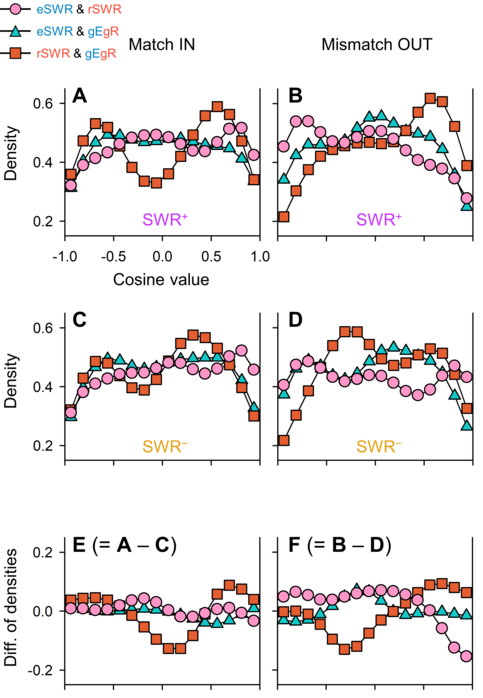
\includegraphics[width=0.5\textwidth]{./src/figures/.png/Figure_ID_07.png}
        	\caption{\DIFdelbeginFL \textbf{\DIFdelFL{Directions of Neural Trajectories during SWRs Based on Encoding and Retrieval States
}}
%DIFAUXCMD
\DIFdelendFL \DIFaddbeginFL \textbf{
\DIFaddFL{Directionality of Neural Trajectories in SWR Based on Encoding and Retrieval States
}}
\DIFaddendFL \smallskip
\\
\textbf{\textit{A--B}} \DIFaddbeginFL \DIFaddFL{Depicted are the }\DIFaddendFL Kernel \DIFdelbeginFL \DIFdelFL{density estimation }\DIFdelendFL \DIFaddbeginFL \DIFaddFL{Density Estimation }\DIFaddendFL (KDE) distributions of $\protect\overrightarrow{{\mathrm{eSWR^+}}} \cdot \protect\overrightarrow{{\mathrm{rSWR^+}}}$ (\textit{pink circles}), $\protect\overrightarrow{{\mathrm{eSWR^+}}} \cdot \protect\overrightarrow{{\mathrm{g_{E}g_{R}}}}$ (\textit{blue triangles}), and $\protect\overrightarrow{{\mathrm{rSWR^+}}} \cdot \protect\overrightarrow{{\mathrm{g_{E}g_{R}}}}$ (\textit{red rectangles}) in Match \DIFdelbeginFL \DIFdelFL{In }\DIFdelendFL \DIFaddbeginFL \DIFaddFL{IN }\DIFaddendFL (\textit{A}) and Mismatch OUT tasks (\textit{B})\DIFaddbeginFL \DIFaddFL{~\mbox{%DIFAUXCMD
\cite{li_functional_2023}}\hspace{0pt}%DIFAUXCMD
}\DIFaddendFL . \textbf{\textit{C--D}} \DIFdelbeginFL \DIFdelFL{Present the corresponding }\DIFdelendFL \DIFaddbeginFL \DIFaddFL{Similar }\DIFaddendFL distributions \DIFdelbeginFL \DIFdelFL{of }\DIFdelendFL \DIFaddbeginFL \DIFaddFL{for these tasks where }\DIFaddendFL $\mathrm{SWR^-}$ \DIFdelbeginFL \DIFdelFL{instead of those of }\DIFdelendFL \DIFaddbeginFL \DIFaddFL{replaces }\DIFaddendFL $\mathrm{SWR^+}$ \DIFdelbeginFL \DIFdelFL{in }\textit{\DIFdelFL{A}} %DIFAUXCMD
\DIFdelFL{and }\textit{\DIFdelFL{B}}%DIFAUXCMD
\DIFdelendFL \DIFaddbeginFL \DIFaddFL{have been presented~\mbox{%DIFAUXCMD
\cite{dimakopoulos_information_2022}}\hspace{0pt}%DIFAUXCMD
}\DIFaddendFL . \textbf{\textit{E--F}} \DIFdelbeginFL \DIFdelFL{Depict the differences in }\DIFdelendFL \DIFaddbeginFL \DIFaddFL{Distinctions between }\DIFaddendFL the distributions of $\mathrm{SWR^+}$ and $\mathrm{SWR^-}$ \DIFdelbeginFL \DIFdelFL{, illuminating }\DIFdelendFL \DIFaddbeginFL \DIFaddFL{highlight }\DIFaddendFL the SWR components (\textit{E} = \textit{C} $-$ \textit{A}; \textit{F} = \textit{D} $-$ \textit{B})\DIFdelbeginFL \DIFdelFL{. Note }\DIFdelendFL \DIFaddbeginFL \DIFaddFL{, where }\DIFaddendFL the biphasic distributions of $\protect\overrightarrow{{\mathrm{rSWR^-}}} \cdot \protect\overrightarrow{{\mathrm{g_{E}g_{R}}}}$ \DIFdelbeginFL \DIFdelFL{, suggesting fluctuations }\DIFdelendFL \DIFaddbeginFL \DIFaddFL{indicate neural oscillations }\DIFaddendFL between \DIFdelbeginFL \DIFdelFL{the }\DIFdelendFL encoding and retrieval states during the Sternberg task\DIFaddbeginFL \DIFaddFL{~\mbox{%DIFAUXCMD
\cite{borders_hippocampus_2022}}\hspace{0pt}%DIFAUXCMD
}\DIFaddendFL . \DIFdelbeginFL \DIFdelFL{Moreover}\DIFdelendFL \DIFaddbeginFL \DIFaddFL{Contrarily}\DIFaddendFL , \DIFaddbeginFL \DIFaddFL{the Mismatch OUT task showed an }\DIFaddendFL inverse \DIFdelbeginFL \DIFdelFL{directionality }\DIFdelendFL \DIFaddbeginFL \DIFaddFL{relationship }\DIFaddendFL between $\protect\overrightarrow{{\mathrm{eSWR^+}}}$ and $\protect\overrightarrow{{\mathrm{rSWR^+}}}$ \DIFdelbeginFL \DIFdelFL{was observed }\DIFdelendFL (\textit{pink circles})\DIFdelbeginFL \DIFdelFL{in the Mismatch OUT task}\DIFdelendFL , \DIFdelbeginFL \DIFdelFL{but }\DIFdelendFL \DIFaddbeginFL \DIFaddFL{a finding }\DIFaddendFL not \DIFaddbeginFL \DIFaddFL{observed }\DIFaddendFL in the Match IN task \DIFaddbeginFL \DIFaddFL{(}\DIFaddendFL \textbf{\textit{E--F}})\DIFaddbeginFL \DIFaddFL{~\mbox{%DIFAUXCMD
\cite{naber_reciprocal_2001,van_strien_anatomy_2009}}\hspace{0pt}%DIFAUXCMD
}\DIFaddendFL . \DIFdelbeginFL \DIFdelFL{Finally}\DIFdelendFL \DIFaddbeginFL \DIFaddFL{Lastly}\DIFaddendFL , \DIFdelbeginFL \DIFdelFL{shifts }\DIFdelendFL \DIFaddbeginFL \DIFaddFL{transitions }\DIFaddendFL from \DIFdelbeginFL \DIFdelFL{the }\DIFdelendFL retrieval to encoding \DIFdelbeginFL \DIFdelFL{states were evident in }\DIFdelendFL \DIFaddbeginFL \DIFaddFL{for }\DIFaddendFL the SWR components \DIFaddbeginFL \DIFaddFL{were apparent }\DIFaddendFL in both \DIFdelbeginFL \DIFdelFL{the }\DIFdelendFL Match IN and Mismatch OUT tasks (\textit{red rectangles} in \DIFdelbeginFL \textit{\DIFdelFL{E}} %DIFAUXCMD
\DIFdelFL{and }\textit{\DIFdelFL{F}}%DIFAUXCMD
\DIFdelendFL \DIFaddbeginFL \textit{\DIFaddFL{E--F}}\DIFaddendFL )\DIFaddbeginFL \DIFaddFL{~\mbox{%DIFAUXCMD
\cite{niediek_reliable_2016,schomburg_spiking_2012}}\hspace{0pt}%DIFAUXCMD
}\DIFaddendFL .
}
% width=0.5\textwidth
        	\label{fig:07}
        \end{figure*}

%%%%%%%%%%%%%%%%%%%%%%%%%%%%%%%%%%%%%%%%%%%%%%%%%%%%%%%%%%%%%%%%%%%%%%%%%%%%%%%%
%% END
%%%%%%%%%%%%%%%%%%%%%%%%%%%%%%%%%%%%%%%%%%%%%%%%%%%%%%%%%%%%%%%%%%%%%%%%%%%%%%%%

\end{document}
